
\فصل{تعریف مسئله}

\قسمت{مدل سیستم}


%%\قسمت{مدل دستگاه تلفن همراه}

ما مدل سیستم را بر اساس مدل ارائه‌شده در~\cite{tang2020deep}، بر مبنای مجموعه‌ای از گره‌های لبه به شکل مجموعه $N = \set{1, 2, \cdots،N}$ و مجموعه‌ای از دستگاه‌های تلفن همراه را به شکل $M = \set{1, 2, \cdots،M}$ در یک سیستم محاسبات لبه متحرک در نظر می‌گیریم و جهت گسترش روش ارایه شده به توسعه محیط سیستم و چالش‌های موجود، از جمله تأخیر و مصرف انرژی مطابق مدل انرژی در~\cite{zhou2021deep} می‌پردازیم. علاوه بر این، ما بر روی هر قسمت، متشکل از مجموعه‌ای از دوره‌های زمانی $T = \set{1, 2, \cdots،T}$ تمرکز می‌کنیم، به شکلی که هر دوره زمانی، یک ثانیه طول خواهد کشید. در زیر، ما مدل اجزا موجود در دستگاه‌های تلفن همراه و گره‌های محسباتی لبه را همانطور که در شکل~\رجوع{شکل: صف‌بندی} نشان داده‌شده‌است، ارائه می‌دهیم. 



ما بر وظایف محاسباتی دستگاه‌های تلفن همراه تمرکز می‌کنیم، به نحوی که هر وظیفه غیرقابل تقسیم بوده و می‌تواند به صورت محلی پردازش شود و یا به یک گره لبه برای پردازش تخلیه شود. ما فرض می کنیم که در ابتدای هر دوره زمانی\پاورقی{Time Slot}، هر دستگاه‌ تلفن همراه، دارای یک وظیفه جدید، با احتمال وقوع مشخص است. این فرضیه با برخی از آثار موجود سازگار است (به عنوان مثال~\cite{liu2016delay}).

هنگامی که یک دستگاه تلفن همراه دارای یک وظیفه جدید است، ابتدا باید تصمیم بگیرد که آیا این وظیفه را به صورت محلی انجام‌دهد و یا به یک گره لبه تخلیه کند. اگر دستگاه تلفن همراه تصمیم به پردازش محاسبات به صورت محلی گیرد، پس از زمان‌بندی (شکل~\رجوع{شکل: صف‌بندی})، آن وظیفه در صف محاسبات\پاورقی{Computation Queue}، برای پردازش محلی  قرار می‌گیرد. در غیر این صورت، دستگاه تلفن همراه باید تصمیم بگیرد که محاسبات را به کدام‌یک از گره‌های لبه تخلیه کند. سپس برنامه زمان‌بندی، محاسبات را به صف انتقال\پاورقی{Transmission Queue} برای تخلیه قرار می‌دهد. سپس محاسبات تخلیه شده به گره لبه انتخاب شده، از طریق لینک بی‌سیم ارسال می‌شود. برای صف انتقال فرض می‌کنیم که اگر پردازش (یا انتقال) یک وظیفه در یک واحد زمانی تکمیل شود، وظیفه بعدی موجود در صف، در ابتدای واحد زمانی بعد پردازش (یا منتقل) می‌شود. این فرضیه با برخی از آثار موجود، از نظر پویایی صف‌بندی در یک سیستم محاسبات لبه متحرک سازگار است. (به عنوان مثال~\cite{liu2016delay}).






هر گره لبه $n \in \mathcal{N}$، $M$ صف را شامل می‌شود، که هر صف برای دستگاه تلفن همراه $m \in \mathcal{M}$ در نظر گرفته شده‌است. ما فرض می‌کنیم که بعد از تخلیه وظیفه و دریافت توسط گره لبه در دوره زمانی، آن وظیفه در صف محاسبات مربوط به دستگاه تلفن همراه ارسال‌کننده در گره لبه، قرار می‌گیرد.   
اگر یک وظیفه از دستگاه تلفن همراه $m \in \mathcal{M}$ در صف محاسبات آن دستگاه در گره لبه $n \in \mathcal{N}$ و در دوره زمانی $t \in \mathcal{T}$ قرار گیرد، متغیر $K_{m,n}^{edge}(t) \in \IZ_{++}$ را تعریف می‌کنیم که به یک شناسه منحصربه‌فرد برای آن وظیفه اشاره دارد. به طور مشخص اگر وظیفه $K_m(t^{'})$ برای $t^{'} \in \set{1,2, \ldots, t-1}$ به گره لبه $n$ در دوره زمانی $t-1$ فرستاده شود، آنگاه $K_{m,n}^{edge}(t) = K_m(t^{'})$. لازم به ذکر است اگر وظیفه‌ای برای انجام وجود نداشته باشد، در این صورت $K_{m,n}^{edge}(t) = 0$ خواهدبود. همچنین متغیر $\lambda_{m,n}^{\text{E}}(t) \in \Lambda \cup \set{0}$ (بیت) را تعریف می‌کنیم که به اندازه وظیفه ورودی در صف محاسبات دستگاه $m$ در گره لبه $n$ در شروع دوره زمانی $t$ اشاره دارد. 
در ادامه، ابتدا مدل وظیفه و تصمیم تخلیه وظیفه را ارائه می‌دهیم. سپس، صف‌های انتقال و محاسبات را معرفی می‌کنیم.

\شروع{شکل}
\centerimg{queue}{14cm}
\شرح{تصویر صف‌های تشکیل‌شده در دستگاه تلفن همراه $m \in \mathcal{M}$ و در گره لبه $n \in \mathcal{N}$.}
\برچسب{شکل: صف‌بندی}
\پایان{شکل}



\قسمت{مدل وظیفه}

در ابتدای دوره زمانی $t \in T$، اگر دستگاه تلفن همراه $m \in M$ یک وظیفه جدید محاسباتی داشته‌باشد، ما متغیر $K_m(t)\in \IZ_+_+$ را تعریف می‌کنیم، که به شناسه منحصر به فرد برای آن وظیفه اشاره دارد. اگر دستگاه تلفن همراه $m$ در ابتدای دوره زمانی $t$ وظیفه جدیدی در اختیار نداشته باشد، $k_m(t)$ را برای ساده‌سازی برابر با صفر قرار می‌دهیم.

متغیر $\lambda_m(t)$(بیت) را به منظور اشاره به اندازه وظیفه ورودی در دوره زمانی $t$ تعریف می‌کنیم. اگر وظیفه جدید $k_m(t)$ در ابتدای دوره زمانی وجود داشته‌باشد، $\lambda_m(t)$ برابر است با اندازه وظیفه $k_m(t)$. در غیر این صورت، $\lambda_m(t)$ برابر با صفر خواهدبود.

ما اندازه وظیفه را از میان مقادیر مجموعه گسسته $\Lambda = \set{\lambda_1, \lambda_2, \cdots, \lambda_|_\Lambda_|}$، همراه با $|\Lambda|$ مقدار فعال قرار می‌دهیم. از این رو، $\lambda_m(t) \in \Lambda \cup \set{0}$ . علاوه بر این، وظیفه $k_m(t)$ نیاز به یک میزان پیچیدگی محاسباتی دارد که با $\rho_m(t)(t)(t)(t)(t)(t)(t)(t)(t)(t)(t)(t)(t)(t)(t)(t)(t)(t)(t)$(سیکل پردازش پردازنده\پاورقی{CPU Cycle} برای هر بیت) نمایش داده می‌شود که تعداد سیکل مورد نیاز پردازنده، برای پردازش یک واحد از محاسبات استفاده می‌شود. وظیفه $k_m(t)$ دارای یک مهلت\پاورقی{Deadline} انجام است، که با $\Delta(t)$ (در دوره زمانی) نشان داده می‌شود. یعنی اگر کار $k_m(t)$ باشد، تا پایان واحد زمانی $t + \Delta(t) - 1$ به طور کامل پردازش نشده‌باشد، پس از آن بلافاصله منقضی\پاورقی{Drop} می‌شود.


\قسمت{تصمیم‌گیری بارسپاری وظیفه}

اگر دستگاه‌ تلفن همراه $m \in M$، در ابتدای دوره زمانی $t \in T$، وظیفه محاسباتی $k_m(t)$ را در دست داشته‌باشد، سپس نیاز به تصمیم‌گیری تخلیه برای وظیفه $k_m(t)$ به شرح زیر است.

در ابتدا، متغیر دوحالتی $x_m(t) \in \set{0,1}$ را که اشاره به تصمیم‌گیری محل پردازش وظیفه $k_m(t)$ دارد، تعریف می‌کنیم، که بیان‌کننده این است که این وظیفه باید به صورت محلی و یا با تخلیه به یک گره لبه پردازش شود. در حالی‌که تصمیم بر پردازش محلی یا (تخلیه محاسباتی) باشد، $x_m(t)$ را برابر با ۱ (یا ۰) قرار می‌دهیم. در ابتدای دوره زمانی $t$، $\lambda_m(t)x_m(t)$ برابر است با تعداد بیت‌های ورودی در صف محاسبات محلی در دستگاه تلفن همراه $m$، و همچنین $\lambda_m(t)(1-x_m(t))$ برابر است با تعداد بیت‌های قرارگرفته در صف انتقال دستگاه $m$.

اگر وظیفه $k_m(t)$ به یک گره لبه تخلیه شود، متغیر باینری $y_m_,_n(t) \in \set{0,1}$ تعریف می‌شود که به محل تخلیه در بین گره‌های لبه اشاره دارد. اگر تصمیم بر تخلیه محاسبات به گره لبه $n$ باشد، متغیر $y_m_,_n(t)$ را برابر با ۱ قرار می‌دهیم, و در غیر این صورت برابر با ۰ خواهدبود. همچنین متغیر $\mathcal{Y}_m(t) = (y_m_,_n(t), n \in \mathcal{N})$ را در اشاره به مجموعه گره‌های لبه تعریف می‌کنیم. شایان ذکر است، برطبق رابطه زیر امکان بارسپاری وظیفه فقط به یک گره از محیط لبه فراهم خواهد بود. 
\begin{alignat}{2}
	\sum_{n \in \mathcal{N}} y_m_,_n(t) = \mathds{1} (x_m(t) = 0), m \in \mathcal{M},  t \in \mathcal{T} 
	\label{100}  
\end{alignat}


\قسمت{مدل ارتباطی}

همانطور که اشاره‌شد، دستگاه‌های تلفن همراه و سرورهای لبه از طریق صف‌ انتقال دستگاه‌ها در ارتباط هستند و به شیوه ورود اول خروج اول فعالیت می‌کند. ورودی‌های این صف وظایفی هستند که برای انجام محاسبات مورد نیازشان تصمیم بر بارسپاری آن‌ها شده‌است. وظایف در انتظار انتقال به گره‌های لبه هستند، که از طریق یک اتصال بی‌سیم در تجهیزات کاربر میسر می‌شود. وظیفه از صف انتقال در دستگاه تلفن همراه به صف محاسبات در گره لبه منتخب منتقل می‌شود. ما یک مدل شبکه بی‌سیم را در نظر می‌گیریم که در آن دستگاه‌های تلفن همراه در کانال‌های متعامد در ارتباط هستند.
 
%اتصالات بی‌سیم بر طبق الگوی~\cite{mao2017stochastic} همراه با محوشدگی در نظر گرفته شده‌اند.

%
%عبارت $|h_{m,n}|^2$ به ظرفیت کانال از دستگاه تلفن همراه $m \in \mathcal{M}$ به گره لبه $n \in \mathcal{N}$ اشاره می‌کند. متغیر $P$ قدرت انتقال تجهیزات کاربر را نشان می‌دهد. نرخ انتقال از دستگاه تلفن همراه $m$ به گره لبه $n$، با متغیر $r\R_{m,n}(t)$(بیت بر ثانیه) نشان داده شده، و بر طبق رابطه زیر محاسبه می‌شود.
%\begin{alignat}{2}
%	r\R_{m,n}(t) = W \log_2(1 + {|h_{m,n}|^2 P \over \sigma^2}) , m \in \mathcal{M}, n \in \mathcal{N}
%	\label{101}  
%\end{alignat}
%%%

%در عبارت بالا، $W$ به پهنای باند تخصیص یافته به کانال اشاره دارد، و $\Delta(t)^2$ نویز دریافتی در گره لبه را بیان می‌کند. مقدار $r\R_{m,n}(t)$ ثابت در نظر گرفته شده‌است. 

در ابتدای دوره زمانی $t \in \mathcal{T}$، اگر وظیفه $k_m(t)$ در صف انتقال برای تخلیه محاسباتی قرار داشته‌باشد، ما متغیر $l_m^{\text{T}}(t) \in \mathcal{T}$ را تعریف می‌کنم که به دوره زمانی که وظیفه $k_m(t)$ ارسال و یا منقضی می‌شود، اشاره دارد. اگر صف انتقال خالی بود و یا $K_m(t)=0$ بود، آنگاه $l_m^{\text{T}}(t) = 0$. 
متغیر $\Delta(t)_m^{\text{T}}(t)$ را برای اشاره به تعداد دوره زمانی که وظیفه $k_m(t)$ باید در انتظار ارسال در صف انتقال بماند، تعریف می‌کنیم. مقدار متغیر $\Delta(t)_m^{\text{T}}(t)$ دستگاه تلفن همراه $m$ قبل از تصمیم‌گیری برای جایگذاری وظیفه در هر یک از صف‌ها، محاسبه می‌کند. متغیر $l_m^{\text{T}}(t^{'})$ را برای $t^{'} < t$ در نظر می‌گیریم، و سپس بر طبق رابطه زیر مقدار $\Delta(t)_m^{\text{T}}(t)$ محاسبه می‌شود. 
\begin{alignat}{2}
	\Delta(t)_m^{\text{T}}(t) = \left[ \max\limits_{t^{'} \in \set{0,1,\ldots,t-1}} l_m^{\text{T}}(t^{'})-t+1\right]^+
	\label{102}  
\end{alignat}



برای سادگی $\Delta(t)^{tran}(0)$ را برابر با صفر در نظر می‌گیریم.
اگر دستگاه $m \in \mathcal{M}$ وظیفه $k_m(t)$ را در دوره زمانی $t \in \mathcal{T}$ در صف انتقال قرار دهد $(x_m(t) = 0)$، آنگاه وظیفه $k_m(t)$ در دوره زمانی $\Delta(t)_m^{\text{T}}(t)$ بر طبق رابطه زیر محاسبه می‌شود.
\begin{alignat}{2}
	l_m^{\text{T}}(t) = \min \set{t + \Delta(t)^{\text{T}(t) + \ceil{D_m^{\text{T}}(t)} - 1, t + \Delta(t) - 1}
	\label{103}  
\end{alignat}

در رابطه بالا متغیر $D_m^{\text{T}}(t)$، در اشاره به زمان  مورد نیاز برای انتقال وظیفه  $k_m(t)$ از دستگاه $m \in \mathcal{M}$ به گره لبه $n \in \mathcal{N}$، به شکل رابطه زیر تعریف شده‌است. 
\begin{alignat}{2}
	D_m^{\text{T}}(t) =  \sum_{n \in \mathcal{N}} {y_{m,n}(t)\lambda_m(t) \over r\R_{m,n}(t)\tau}
	\label{104}  
\end{alignat}

از این رو بخش اول عملگر کمینه برابر است با دوره زمانی که وظیفه $k_m(t)$ کاملا منتقل شده‌باشد در حالی که مهلتش به پایان نرسد، و بخش دوم نیز به دوره زمانی اشاره دارد که وظیفه $k_m(t)$ منقضی و دورریخته می‌شود. در نتیجه، $l_m^{\text{T}}(t)$ دوره زمانی را که وظیفه $k_m(t)$ به طور کامل به گره لبه $n \in \mathcal{M}$ منتقل شود را بیان می‌کند. 

ما همچنین جهت ارزیابی مصرف انرژی سیستم، متغیر ${E_m^{tran}}$ را در اشاره به انرژی مصرفی مربوط به انتقال وظیفه $k_m(t)$ از دستگاه $m \in \mathcal{M}$ به گره لبه $n \in \mathcal{M}$ برطبق رابطه زیر تعریف می‌کنیم.  
\begin{alignat}{2}
	E_m^{\text{T}}(t) = D_m^{\text{T}}(t)  \mathcal{P}^{\tetx{T}} \tau =  \sum_{n \in \mathcal{N}} {y_{m,n}(t)\lambda_m(t) \over \R_{m,n}(t) \mathcal{P}^{\tetx{T}}  
	\label{105}  
\end{alignat}








در رابطه بالا مقدار ثابت $\mathcal{P}^{\tetx{T}} $ را به عنوان نیروی انتقال مصرفی در زمان استفاده کامل از ظرفیت لینک ارتباطی دستگاه $m \in \mathcal{M}$ در نظر می‌گیریم. 

\قسمت{مدل محاسباتی}
\زیرقسمت{محاسبات محلی}



همانطور که اشاره‌شد، صف محاسبات در دستگاه تلفن همراه محل قرارگیری وظایفی خواهدبود که نتیجه تصمیم‌گیری برای محل پردازش آن‌ها به صورت محلی و با استقاده از منابع موجود در تجهیزات کاربر تعیین شده‌است. سیاست جای‌گیری در صف محاسبات به شکل اولین ورود، اولین خروج\پاورقی{First-in First-out} در نظر گرفته‌شده‌ و ورودی‌ها وظایفی هستند که به صورت محلی پردازش می‌شوند. ما یک پردازنده در جهت محاسبات وظایف موجود در صف در نظر می‌گیریم. متغیر $f_m^{\text{T}}$ (سیکل پردازنده در هر ثانیه) به ظرفیت محاسباتی پردازنده در دستگاه $m \in \mathcal{M}$ اشاره می‌کند، و مقداری  ثابت خواهدبود.      

در شروع دوره زمانی $t \in \mathcal{T}$، اگر وظیفه $k_m(t)$ در صف محاسبات قرار داشته‌باشد، ما متغیر $l_m^{\text{C}}(t) \in \mathcal{T}$ را تعریف می‌کنیم که نشان‌دهنده دوره زمانی خواهدبود که وظیفه $k_m(t)$ انجام و یا دورریخته شده‌باشد. اگر در ابتدای دوره زمانی $t \in \mathcal{T}$ ، صف محاسبات خالی باشد و یا $K_m(t)=0$ ،  $l_m^{\text{C}}(t) = 0$ قرار می‌دهیم. 

متغیر $\Delta(t)_m^{\text{C}}(t)$ (در دوره زمانی) را به منظور اشاره به تعداد دوره زمانی باقی‌مانده تا پردازش برای وظیفه $k_m(t)$ در صف محاسبات تعریف می‌کنیم. لازم به ذکر است که دستگاه $m$ مقدار متغیر $\Delta(t)_m^{\text{C}}(t)$ را قبل از تصمیم‌گیری و جایگیری وظیفه در صف، محاسبه می‌کند. متغیر $l_m^{\text{C}}(t^{'})$ را در $t^{'} > t$ در نظر می‌گیریم، و مطابق با رابطه زیر مقدار $\Delta(t)_m^{\text{C}}(t)$ محاسبه می‌شود. 
\begin{alignat}{2}
	\Delta(t)_m^{\text{C}}(t) = \left[ \max\limits_{t^{'} \in \set{0,1,\ldots,t-1}} l_m^{\text{C}}(t^{'})-t+1 \right]^+
	\label{106}  
\end{alignat}



در رابطه بالا عملگر $[z]^+ = \max \set{0,z}$، و متغیر $l_m^{\text{C}}(0) = 0$ است. به طور مشخص عبارت $\max_{t^{'} \in \set{0,1,2,\ldots, t-1}}l_m^{\text{C}}(t^{'})$، دوره زمانی که تمامی وظایف جای‌گرفته در صف، به سرانجام رسیده‌اند را تا قبل از دوره زمانی $t$ تعیین می‌کند. از این رو، $\Delta(t)_m^{\text{C}}(t)$ تعداد دوره زمانی که وظیفه $k_m(t)$ باید در انتظار پردازش باشد را نشان می‌دهد. به عنوان مثال، فرض کنید وظیفه $K_m(1)$ در صف محاسبات محلی قرار دارد، و پردازش آن در دوره زمانی ۵ کامل خواهدشد. بنابراین $l_m^{\text{C}}(1) = 5$ یعنی آن وظیفه باید $\Delta(t)^{comp}(3) = [\max \set{5,0}-3+1]^+ = 3$ دوره زمانی در انتظار اتمام فرآیند، بماند.

اگر دستگاه $m \in \mathcal{M}$  در ابتدای دوره زمانی $t \in \mathcal{T}$، وظیفه $k_m(t)$ را در صف محاسبات محلی قراردهد ($x_m(t) = 1$)، آنگاه وظیفه $k_m(t)$ در دوره زمانی $l_m^{\text{C}}(t)$ پردازش شده و یا از بین رفته است:  
\begin{alignat}{2}
	l_m^{\text{C}}(t) = \min \set{t + \Delta(t)_m^{\text{C}}(t) + \ceil{D_m^{\text{C}}(t)} - 1, t + \Delta(t) - 1}
	\label{107}  
\end{alignat}

در رابطه بالا متغیر $D_m^{\text{C}}(t)$ در اشاره به زمان  مورد نیاز برای پردازش کامل وظیفه  $k_m(t)$ در دستگاه $m \in \mathcal{M}$، مطابق با رابطه زیر تعریف می‌شود.
\begin{alignat}{2}
	D_m^{\text{C}}(t) = { \lambda_m(t)  \over  f_m^{\text{T}}  \tau /  \rho_m(t)(t)(t)(t)(t)(t)(t)(t)(t)(t)(t)(t)(t)(t)(t)(t)(t)(t)(t)}
	\label{108}  
\end{alignat}

به طور مشخص، پردازش وظیفه $k_m(t)$ در دوره زمانی $t + \Delta(t)_m^{\text{C}}(t)$ آغاز خواهدشد. از این رو بخش اول عملگر کمینه برابر است با دوره زمانی که وظیفه $k_m(t)$ کامل انجام شده‌باشد در حالی که مهلتش به پایان نرسد، و بخش دوم نیز به دوره زمانی اشاره دارد که وظیفه $k_m(t)$ منقضی و دورریخته می‌شود. در نتیجه، $l_m^{\text{C}}(t)$ دوره زمانی را که وظیفه $k_m(t)$ به سرانجام خواهد رسید را بیان می‌کند. 

همچنین جهت ارزیابی مصرف انرژی سیستم، مقدار ثابت $\mathcal{P}^{\text{T}}(t) $ را به عنوان نیروی مصرفی در حالت استفاده کامل از ظرفیت پردازنده دستگاه $m \in \mathcal{M}$ در نظر می‌گیریم و متغیر $E_m^{\text{L}}(t))$ را در اشاره به انرژی مصرفی مربوط به پردازش کامل وظیفه $k_m(t)$ در دستگاه $m \in \mathcal{M}$ برطبق رابطه زیر تعریف می‌کنیم.
\begin{alignat}{2}
	E_m^{\text{L}}(t)) =  D_m^{\text{C}}(t) \mathcal{P}^{\text{T}}(t)  \tau =  {\mathcal{P}^{\text{T}}(t) \lambda_m(t) \rho_m(t)(t)(t)(t)(t)(t)(t)(t)(t)(t)(t)(t)(t)(t)(t)(t)(t)(t)(t)  \over  f_m^{\text{T}}}
	\label{109}  
\end{alignat}


\زیرقسمت{محاسبات در لبه}


در اینجا نیز صف در ارتباط با یک دستگاه تلفن همراه که در یک گره لبه مستقر است، به شیوه ورود اول خروج اول عمل می‌کند. ورودی صف‌ها، وظایف تخلیه شده توسط دستگاه تلفن همراه به آن گره لبه است. متغیر $\eta_{m,n}^{\text{E}}(t)$ (بیت) را در اشاره به طول صف دستگاه تلفن همراه $m \in \mathcal{M}$، در گره لبه $n \in \mathcal{N}$، و در انتهای دوره زمانی $t \in \mathcal{T}$، تعریف می‌کنیم. در میان صف‌های گره لبه اگر در ابتدای دوره زمانی $t$، وظیفه ورودی در صف دستگاه تلفن همراه $m$ وجود داشته‌باشد ($\lambda_{m,n}^{\text{E}}(t)>0$) و یا وظیفه‌ای از دوره زمانی قبلی باقی مانده باشد ($\eta_{m,n}^{\text{E}}(t-1)>0$)، به آن صف به عنوان یک صف فعال در آن گره در دوره زمانی $t$ اشاره می‌کنیم. همچنین متغیر $\mathcal{B}_n(t)$ را برای اشاره به مجموعه صف‌های فعال در گره لبه $n$ در دوره زمانی $t$ را بر طبق رابطه زیر تعریف می‌کنیم.
\begin{alignat}{2}
	\mathcal{B}_n(t) = \set{m \ | \ m \in \mathcal{M}, \lambda_{m,n}^{\text{E}}(t)>0 \ or \,  \eta_{m,n}^{\text{E}}(t-1)>0}
	\label{110}  
\end{alignat}


متغیر $B_n(t)$ را نیز در اشاره به تعداد صف‌های فعال در گره لبه $n \in \mathcal{N}$، در دوره زمانی $t \in \mathcal{T}$ به شکل $B_n(t)=|\mathcal{B}_n(t)|$ تعریف می‌کنیم. 

در هر دوره زمان $t \in \mathcal{T}$، صف‌های فعال در گره لبه $n \in \mathcal{N}$، که در مجموعه $\mathcal{B}_n(t)$ قرار دارند، ظرفیت محاسباتی آن گره لبه را با یکدیگر بر اساس روش عمومی اشتراک‌گذاری پردازنده~\cite{parekh1993generalized}، تقسیم می‌کنند. متغیر $f_n^{\text{E}}$ را در اشاره به ظرفیت محاسباتی گره لبه $n$ تعریف می‌شود. از این رو گره لبه $n$ می‌تواند به مقدار $f_n^{\text{E}}/(\rho_m(t)(t)(t)(t)(t)(t)(t)(t)(t)(t)(t)(t)(t)(t)(t)(t)(t)(t)(t) B_n(t))$، ظرفیت محاسباتی به هر دستگاه فعال متصل $m \in \mathcal{B}_n(t)$ در دوره زمانی $t$ تخصیص‌دهد.
برای هر صف در گره لبه ، فرض می‌کنیم که اگر
پردازش یک وظیفه در یک دوره زمانی تکمیل شود، وظیفه بعدی در صف، در ابتدای دوره زمانی بعدی پردازش می‌شود. برای محاسبه طول صف محاسبات دستگاه $m \in \mathcal{M}$ در گره لبه $n \in \mathcal{T}$، متغیر $e_{m,n}^{\text{E}}(t)$(بیت) را در اشاره به تعداد وظایف منقضی‌شده توسط این صف در پایان دوره زمانی $t \in \mathcal{T}$، بیان می‌کنیم. در نتیجه طول  صف $\eta_{m,n}^{\text{E}}(t)$ از رابطه زیر به‌روز خواهدشد.  
\begin{alignat}{2}
	\eta_{m,n}^{\text{E}}(t)= 
	\left[\eta_{m,n}^{\text{E}}(t-1) + \lambda_{m,n}^{\text{E}}(t) - {f_n^{\text{E}}\over \rho_m(t)(t)(t)(t)(t)(t)(t)(t)(t)(t)(t)(t)(t)(t)(t)(t)(t)(t)(t)B_n(t)}\mathds{1}(m \in \mathcal{B}_n(t)) - e_{m,n}^{\text{E}}(t)\right]^+
	\label{111}  
\end{alignat}


به طور خاص اندازه صف $\eta_{m,n}^{\text{E}}(t)$ برابر است با طول صف در انتهای دوره زمانی  $\eta_{m,n}^{\text{E}}(t-1)$ به اضافه تفاوت بین وظایف ورودی و وظایف به پایان رسیده (انجام یا منقضی شده) در دوره زمانی $t$. 

همچنین جهت محاسبه انرژی مصرفی مربوط به وظایف بارسپاری شده، متغیر $D_{m,n}^{\text{E}}(t)$ را در اشاره به زمان پردازش وظیفه $k_m(t)$ در گره لبه $n \in \mathcal{N}$ مطابق با رابطه زیر تعریف می‌کنیم. 
\begin{alignat}{2}
	D_{m,n}^{\text{E}}(t) = { \lambda_{m,n}^{\text{E}}(t) \rho_m(t)(t)(t)(t)(t)(t)(t)(t)(t)(t)(t)(t)(t)(t)(t)(t)(t)(t)(t) \over  \mathcal{B}_n(t)f_n^{\text{E}} \tau}
	\label{112}  
\end{alignat}

در پی آن مقدار ثابت $\mathcal{P}^{\text{E}}$ را برابر با مقدار انرژی مصرفی پردازنده لبه در حالت استفاده کامل از ظرفیت در نظر می‌گیریم و متفیر $e_{m,n}^{\text{E}}(t)$ را در اشاره به انرژی مصرفی پردازش وظیفه $k_m(t)$ در گره لبه $n \in \mathcal{N}$ طبق رابطه (۴-۲۴) تعریف می‌کنیم. 
\begin{alignat}{2}
	e_{m,n}^{\text{E}}(t) = D_{m,n}^{\text{E}}(t) \mathcal{B}_n(t) \mathcal{P}^{\text{E}} \tau  = {\mathcal{P}^{\text{E}}  \lambda_{m,n}^{\text{E}}(t) \rho_m(t)(t)(t)(t)(t)(t)(t)(t)(t)(t)(t)(t)(t)(t)(t)(t)(t)(t)(t) \over  f_n^{\text{E}}}
	\label{113}  
\end{alignat}


علاوه بر انرژی مصرفی مربوط به پردازش وظیفه در گره لبه، ما انرژی مصرفی رابط کاربری دستگاه را در زمان انتظار برای تکمیل وظیفه در لبه در نظر می‌گیریم. از این رو مقدار ثابت $\mathcal{P}^{\text{I}}$، برابر با مقدار مصرف انرژی رابط کاربری در زمان انتظار برای دستگاه $m \in \mathcal{M}$ را بیان‌کرده و متغیر $E_{m,n}^{\text{I}}(t)$ را در اشاره به مقدار مصرف انرژی مربوط به رابط کاربری دستگاه $m \in \mathbb{M}$ در زمان انتظار برای تکمیل و بازگشت وظیفه $k_m(t)$ از گره لبه بر طبق رابطه (۴-۲۵) تعریف می‌کنیم.
\begin{alignat}{2}
	E_m^{idle}(t) = D_{m,n}^{\text{E}}(t) \mathcal{P}^{\text{I}} \tau  = {\mathcal{P}^{\text{I}}  \lambda_{m,n}^{\text{E}}(t) \rho_m(t)(t)(t)(t)(t)(t)(t)(t)(t)(t)(t)(t)(t)(t)(t)(t)(t)(t)(t) \over \mathcal{B}_n(t)  f_n^{\text{E}} }
	\label{114}  
\end{alignat}

بر این اساس ما برای محاسبه کامل انرژی مصرفی مربوط به بارسپاری وظیفه $k_m(t)$، انرژی مصرفی محاسبه‌شده در (۴-۶) ، (۴-۱۴) و (۴-۱۵) را تجمیع می‌کنیم، که شامل انرژی مصرفی برای جابه‌جایی وظیفه از دستگاه $m \in \mathcal{M}$ به گره لبه $n \in \mathcal{N}$ $(E_m^{\text{T}}(t))$، انرژی مصرفی محاسبات مربوطه در گره لبه $(e_{m,n}^{\text{E}}(t))$ و انرژی مصرفی رابط کاربری $(E_m^{idle}(t))$ می‌باشد. از این رو متغیر $E_m^{offl}(t)$ را در اشاره به انرژی مصرف شده در کل فرآیند بارسپاری وظیفه $k_m(t)$ در زمان $t \in \mathcal{T}$، بر طبق رابطه زیر تعریف می‌کنیم. 
\begin{align}{}
	\left E_m^{offl}(t)
	&=\left e_{m,n}^{\text{E}}(t)  + E_m^{trans}(t)  + E_m^{idle}(t)  \\
	&= {\mathcal{P}^{\text{E}}  \lambda_{m,n}^{\text{E}}(t) \rho_m(t)(t)(t)(t)(t)(t)(t)(t)(t)(t)(t)(t)(t)(t)(t)(t)(t)(t)(t) \over  f_n^{\text{E}}} +  {\mathcal{P}^{\tetx{T}}  \lambda_{m}(t) \over \R_{m,n}(t) + {\mathcal{P}^{\text{I}}  \lambda_{m,n}^{\text{E}}(t) \rho_m(t)(t)(t)(t)(t)(t)(t)(t)(t)(t)(t)(t)(t)(t)(t)(t)(t)(t)(t) \over \mathcal{B}_n(t)  f_n^{\text{E}} }
	\tag*{}
\end{align}

بنابراین ما مقدار انرژی مصرفی در هر لحظه از زمان را برای هر یک از دستگاه‌های هوشمند به شکل زیر محاسبه می‌کنیم.
$ E_m(t) = x_m(t) E_m^{\text{L}}(t))+ (1 - x_m(t))  E_m^{offl}(t) = \\$
$$ x_m(t) \bigg( {\mathcal{P}^{\text{T}}(t) \lambda_m(t) \rho_m(t)(t)(t)(t)(t)(t)(t)(t)(t)(t)(t)(t)(t)(t)(t)(t)(t)(t)(t)  \over  f_m^{\text{T}}} \bigg) + (1 - x_m(t)) \bigg( {\mathcal{P}^{\text{E}}  \lambda_{m,n}^{\text{E}}(t) \rho_m(t)(t)(t)(t)(t)(t)(t)(t)(t)(t)(t)(t)(t)(t)(t)(t)(t)(t)(t) \over  f_n^{\text{E}}} +  {\mathcal{P}_m \lambda_{m}(t) \over \R_{m,n}(t) + {\mathcal{P}^{\text{I}} \lambda_{m,n}^{\text{E}}(t) \rho_m(t)(t)(t)(t)(t)(t)(t)(t)(t)(t)(t)(t)(t)(t)(t)(t)(t)(t)(t) \over \mathcal{B}_n(t)  f_n^{\text{E}} } \bigg)$$
 \begin{align}{}
	\label{115}
\end{align}



\زیرقسمت{پردازش و انقضا وظیفه}


اگر وظیفه $K_{m,n}^{edge}(t)$ از دستگاه تلفن همراه $m \in \mathcal{M}$ در ابتدای دوره زمانی $t \in \mathcal{T}$ در صف محاسبات متناظر آن دستگاه، در گره لبه $n \in \mathcal{N}$ قرار داشته‌باشد، متغیر $l_{m,n}^{edge}(t) \in \mathcal{T}$ برای اشاره به دوره زمانی که این وظیفه به سرانجام می‌رسد، تعریف می‌شود. با توجه به بار محاسباتی نامعلوم آینده در گره لبه $n$، مقدار متغیر $l_{m,n}^{edge}(t)$ تا زمانی که وظیفه $K_{m,n}^{edge}(t)$ به سر انجام رسد، نامشخص خواهدبود. اگر $K_{m,n}^{edge}(t)=0$ باشد، آنگاه $l_{m,n}^{edge}(t)=0$ خواهدبود. 
برای تعریف متغیر $l_{m,n}^{edge}(t)$، متغیر $\hat{l}_{m,n}^{edge}(t)$ را در اشاره به دوره زمانی که پردازش وظیفه $K_{m,n}^{edge}(t)$ آغاز می‌شود، بر طبق رابطه زیر در نظر می‌گیریم. 
\begin{alignat}{2}
	\hat{l}_{m,n}^{edge}(t) = \max \set{t, \max\limits_{t^{'} \in \set{0,1,\ldots,t-1}}l_{m,n}^{edge}(t^{'})+1}
	\label{116}  
\end{alignat}


به طور مشخص می‌دانیم دوره زمانی که وظیفه $K_{m,n}^{edge}(t)$ آغاز می‌شود، نباید از دوره زمانی که وظیفه در صف مستقر می‌شود، نزدیک‌تر باشد. همچنین می‌دانیم دوره زمانی که هر وظیفه وارد سیستم می‌شود باید قبل از زمان پردازش و یا انقضا آن وظیفه باشد. 
با توجه به تحقق سطوح بار در گره لبه $n$، $l_{m,n}^{edge}(t)$ دوره زمانی را بر طبق محدودیت‌های زیر بیان خواهدکرد. 
\begin{alignat}{2}
	\sum_{t^{'}=\hat{l}_{m,n}^{edge}(t)}^{l_{m,n}^{edge}(t)}{f_n^{\text{E}} \over \rho_m(t)(t)(t)(t)(t)(t)(t)(t)(t)(t)(t)(t)(t)(t)(t)(t)(t)(t)(t)B_n(t^{'})}\mathds{1}(m \in \mathcal{B}_n(t^{'})) \geqslant \lambda_{m,n}^{\text{E}}(t)
	\label{117}  
\end{alignat}
\begin{alignat}{2}
	\sum_{t^{'}=\hat{l}_{m,n}^{edge}(t)}^{l_{m,n}^{edge}(t)-1}{f_n^{\text{E}} \over \rho_m(t)(t)(t)(t)(t)(t)(t)(t)(t)(t)(t)(t)(t)(t)(t)(t)(t)(t)(t)B_n(t^{'})}\mathds{1}(m \in \mathcal{B}_n(t^{'})) < \lambda_{m,n}^{\text{E}}(t)
	\label{118}  
\end{alignat}






\فصل{مسئله بارسپاری وظیفه مبتنی بر یادگیری تقویتی عمیق}

در این بخش، چالش تخلیه محاسباتی را مورد بررسی قرار می‌دهیم و مدل بارسپاری وظیفه مبتنی بر یادگیری تقویتی عمیق را در سیستم محاسبات لبه متحرک ارائه می‌دهیم. 

\قسمت{بیان مسئله با یادگیری تقویتی عمیق}


به طور خاص، در ابتدای هر دوره زمانی، هر دستگاه تلفن همراه حالت وضعیت خود را (به عنوان مثال، اندازه وظیفه، اطلاعات صف) را مشاهده می‌کند. اگر یک وظیفه جدید تازه واردشده برای پردازش، وجود داشته‌باشد، دستگاه تلفن همراه اقداماتی را برای انجام این وظیفه باید انتخاب کند. حالت مشاهده‌شده و اقدام انتخاب شده باعث ایجاد هزینه (به عنوان مثال، تأخیر وظیفه و مصرف انرژی) برای دستگاه تلفن همراه خواهدشد. هدف هر دستگاه تلفن همراه این است که هزینه‌های طولانی مدت خود را با بهینه‌سازی سیاست تصمیم‌گیری و نقشه‌برداری از مدل سیستم، به حداقل برساند. در زیر، ابتدا حالت، عمل و هزینه را معرفی می‌کنیم، و سپس تابع هزینه را برای هر دستگاه فرموله می‌کنیم.

\زیرقسمت{حالت}
در شروع دوره زمانی $t \in \mathcal{T}$، هر دستگاه $m \in \mathcal{M}$ اطلاعات حالت جاری شامل اندازه وظیفه ورودی، اطلاعات صف‌ها و اطلاعات تاریخی از سطح بار گره‌های لبه را مشاهده می‌کند. به طور خاص، دستگاه تلفن همراه $m$ دارای بردار حالت زیر است: 
\begin{alignat}{2}
	\mathcal{S}_m(t)=\Big(\lambda_m(t), \Delta(t)_m^{\text{C}}(t), \Delta(t)^{\text{T}(t), \textbf{\textit{q}}_m^{edge}(t-1), \textbf{\textit{H}}(t), \mathcal{\omega}_m(t) \Big)
	\label{50}  
\end{alignat}


در رابطه بالا بردار $\textbf{\textit{q}}_m^{edge}(t-1) = (\eta_{m,n}^{\text{E}}(t-1), n) \in \mathcal{N}$ بوده، و ماتریس $\textbf{\textit{H}}(t)$ شامل اطلاعات تاریخی از سطح بار (تعداد صف‌های فعال) گره‌های لبه در طول $T^{step}$ (از دوره زمانی $t-T^{step}$ تا دوره زمانی $t-1$) دوره زمانی گذشته است. همراه با اطلاعات تاریخی از سطح بار محاسباتی گره‌های لبه می‌توانیم وضعیت سطح بار آن‌ها را در آینده نزدیک تخمین بزنیم. این اطلاعات، تحت ماتریسی به اندازه $T^{step} \times N$ در نظر گرفته می‌شوند. عبارت $\set{\textbf{\textit{H}}(t)}_{i,j}$ را در اشاره به هر یک از مقادیر ماتریس $\set{\textbf{\textit{H}}(t)}$ تعریف می‌کنیم، که متناظر با سطح بار محاسباتی هر گره لبه در یک دوره زمانی است. مقادیر ماتریس $\set{\textbf{\textit{H}}(t)}$ بر طبق رابطه زیر محاسبه می‌شوند.
\begin{alignat}{2}
	\set{\textbf{\textit{H}}(t)}_{i,j} = B_j(t - T^{step} + i -1)
	\label{51}  
\end{alignat}


متغیر $\mathcal{S}$ را به شکل مجموعه فضای حالت گسسته متناهی برای هر دستگاه تلفن همراه تعریف می‌کنیم. مجموعه $\mathcal{S} = \Lambda \times \set{0,1,\ldots,T}^2 \times \mathcal{Q}^N \times \set{0,1,\ldots,M}^{T^{step} \times N}$ است به نحوی که $\mathcal{Q}$ به مجموعه مقادیر فعال برای طول صف در گره لبه و در طول دوره‌های زمانی اشاره دارد. 
دستگاه تلفن همراه $m \in \mathcal{M}$ می‌تواند اطلاعات حالت $\lambda_m(t)$، $\Delta(t)_m^{\text{C}}(t)$ و $\Delta(t)_m^{\text{T}}(t)$ را به صورت محلی در ابتدای دوره زمانی $t$ محاسبه کند. همچنین دستگاه تلفن همراه $m$ می‌تواند بردار اطلاعات حالت $\textbf{\textit{q}}_m^{edge}(t-1)$ را از طریق تعداد بیت‌های ارسال‌شده از دستگاه $m$ به هر گره لبه در هر دوره زمانی و تعداد بیت‌های پردازش و یا منقضی شده در هر دوره زمانی، مطابق با رابطه (۸) محاسبه‌کند. برای ماتریس $\textbf{\textit{H}}(t)$ فرض می‌کنیم که هر گره لبه تعداد صف‌های فعال خود را در انتهای هر دوره زمانی منتشر می‌کند.از آنجا که تعداد صف‌های فعال همیشه یک عدد کوچک است، و می‌تواند توسط چندین بیت نشان داده‌شود، انتشار این مقادیر تنها  سربار کوچکی بر سیستم تحمیل خواهدکرد.


\زیرقسمت{عمل}
در شروع دوره زمانی $t \in \mathcal{T}$، اگر دستگاه تلفن همراه $m \in \mathcal{M}$ یک وظیفه جدید ورودی $k_m(t)$ داشته‌باشد، در این صورت دستگاه تلفن همراه باید در مورد جایگاه پردازش وظیفه، در موارد زیر تصمیم‌گیری انجام‌دهد

\شروع{فقرات}
\فقره  محاسبات وظیفه به صورت محلی انجام‌گیرد و یا به گره‌های لبه بارسپاری شود $x_m(t)$.

\فقره در صورت بارسپاری وظیفه، وظیفه مورد نظر به کدام‌یک از گره‌های لبه انتقال داده‌شود $y_m(t)$.

\پایان{فقرات}


از این‌رو، عمل در دستگاه تلفن همراه $m$ در دوره زمانی $t$ به صورت بردار زیر تعریف می‌شود:
\begin{alignat}{2}
	a_m(t) = (x_m(t), y_m(t))
	\label{52}  
\end{alignat}


همچنین متغیر $\mathcal{A}$ را در اشاره مجموعه فضای عمل تعریف می‌کنیم، $\mathcal{A} = \set{0,1}^{1+N}$. 


\زیرقسمت{هزینه}
اگر یک وظیفه به طور کامل پردازش شده‌باشد، آنگاه تأخیر آن وظیفه، اختلاف زمانی بین ورود و تکمیل محاسبات آن، می‌باشد. متغیر $Delay_m(s_m(t),a_m(t))$ (دوره زمانی) را در اشاره به تأخیر وظیفه $k_m(t)$، در حالت $s_m(t)$ و با عمل $a_m(t)$، بر طبق رابطه زیر تعریف می‌کنیم. 

اگر $x_m(t) = 1$:
\begin{alignat}{2}
	\textsl{Delay}_m(s_m(t),a_m(t)) = l_m^{\text{C}}(t) - t + 1
	\label{53}  
\end{alignat}
\begin{alignat}{2}
	\textsl{Energy}_m(s_m(t),a_m(t)) = E_m^{\text{L}}(t)) 
	\label{54}  
\end{alignat}
اگر $x_m(t) = 0$:
\begin{alignat}{2}
	\textsl{Delay}_m(s_m(t),a_m(t)) = \sum\limits_{n \in \mathcal{N}} \sum\limits_{t^{'}=t}^{T}\mathds{1}(k_{m,n}^{edge}(t^{'}) = k_m(t))l_{m,n}^{edge}(t^{'}) - t +1
	\label{55}  
\end{alignat}
\begin{alignat}{2}
	\textsl{Energy}_m(s_m(t),a_m(t)) = \sum\limits_{n \in \mathcal{N}} \sum\limits_{t^{'}=t}^{T}\mathds{1}(k_{m,n}^{edge}(t^{'}) = k_m(t)) E_{m,n}^{offl}(t^{'}) 
	\label{56}  
\end{alignat}

	$$Average\; QOE= - { \sum_{t \in \mathcal{T}} \sum_{m \in \mathcal{M}} \mathcal{C}_m(t) \big / \mathcal{M} \times \mathcal{T}}$$

به طور مشخص، فرض می‌کنیم، وظیفه $k_m(t)$ در ابتدای دوره زمانی $t$، وارد سیستم شود. اگر وظیفه $k_m(t)$ در صف محاسبات محلی قرارگیرد، آنگاه $l_m^{\text{C}}$ دوره زمانی را نشان می‌دهد که وظیفه پردازش می‌شود. همچنین اگر وظیفه $k_m(t)$ در صف انتقال برای تخلیه محاسباتی قرارگیرد، در این صورت $\sum\limits_{n \in \mathcal{N}} \sum\limits_{t^{'}=t}^{T}\mathds{1}(k_{m,n}^{edge}(t^{'}) = k_m(t))l_{m,n}^{edge}(t^{'})$، دوره زمانی را نشان می‌دهد که وظیفه $k_m(t)$ پردازش می‌شود. در این رابطه عبارت $\mathds{1}(K_{m,n}^{edge}(t^{'}) = K_m(t)) = 1$ نشان‌دهنده این است که وظیفه $k_m(t)$ در صف مربوطه در گره لبه $n \in \mathcal{N}$ در ابتدای دوره زمانی $t^{'}$ قرار دارد، و متغیر $l_{m,n}^{edge}(t^{'})$ دوره زمانی است که وظیفه در صف دستگاه تلفن همراه $m$ در گره لبه $n$ در ابتدای دوره زمانی $t^{'}$ پردازش می‌شود. 
تابع هزینه مربوط به وظیفه $k_m(t)$ را در صورتی که به شکل کامل پردازش شود، به شکل زیر تعریف می‌شود:
\begin{alignat}{2}
	 \textsl{C}_m(s_m(t),a_m(t)) = \alpha \; \textsl{Delay}_m(s_m(t),a_m(t))  +  (1-\alpha) \, \textsl{Energy}_m(s_m(t),a_m(t)) 
	\label{57}  
\end{alignat}

\begin{alignat}{2}
	\textsl{C}_m(s_m(t),a_m(t)) =  \textsl{Battry}_m(t)  \times \Omega  +  (1-\textsl{Battry}_m(t)) \, \textsl{Energy}_m(s_m(t),a_m(t)) 
	\label{57}  
\end{alignat}



و از طرفی اگر وظیفه $k_m(t)$ منقضی شود، تابع هزینه به صورت زیر خواهدبود:
\begin{alignat}{2}
	\textsl{C}_m(s_m(t),a_m(t)) = \Omega
	\label{58}  
\end{alignat}

متغیر $\Omega > 0$ را به عنوان یک مقدار ثابت جریمه برای وظایف از دست‌رفته در نظر می‌گیریم. اگر وظیفه $K_m(t)=0$ باشد، در این صورت متغیر  $\textsl{C}_m(s_m(t),a_m(t))=0$ قرار می‌دهیم. در ادامه برای سادگی از عبارت $\textsl{C}_m(t)$ در اشاره به $\textsl{C}_m(s_m(t),a_m(t))$ استفاده می‌کنیم. 




\قسمت{سیاست بهینه}

سیاست دستگاه $m \in \mathcal{M}$ نقشه‌برداری از حالات و اعمال در محیط می‌باشد ($\pi_m : \mathcal{S} \rightarrow \mathcal{A}$). متغیر $\gamma \in (0,1]$ را که در اشاره به عامل تنزیل\پاورقی{Discount Factor} تابع هزینه در آینده بیان می‌شود، تعریف می‌کنیم. هدف پیدا کردن سیاست بهینه برای هر دستگاه است، به نحوی که هزینه تأخیر و انرژی طولانی مدت در آن به حداقل برسد. 
\begin{alignat}{2}
	\pi_m^* = arg\  \min\limits_{\pi_m}  \mathbb{E} \Bigg[ \sum\limits_{t \in \mathcal{T}}  \gamma^{t-1}c_m(t) \Bigg| \pi_m \Bigg]
	\label{59}  
\end{alignat}


عملگر $\mathbb{E}[.]$ با توجه به پارامترهای سیستمی متغیر زمانی، به عنوان مثال، ورود وظیفه و الزامات محاسباتی وظایف در تمام دستگاه‌های تلفن همراه اشاره دارد. 


\قسمت{الگوریتم بارسپاری وظیفه مبتنی بر یادگیری تقویتی عمیق}
در این بخش، یک الگوریتم تخلیه مبتنی بر یادگیری تقویتی عمیق را ارائه می‌دهیم که هر دستگاه را قادر به تصمیم گیری تخلیه به شکل توزیع‌شده می‌سازد. این الگوریتم بر اساس یادگیری $Q$ عمیق، سیاست بهینه در تصمیم‌گیری تخلیه را تقریب می‌زند. از آنجایی که یادگیری $Q$ عمیق یک روش بدون مدل است، الگوریتم پیشنهادی می‌تواند تنظیمات پیچیده سیستم و تعامل بین دستگاه‌های تلفن همراه را بدون دانش قبلی از محیط سیستم و پویایی تعامل، بررسی‌کند. در همین حال، الگوریتم پیشنهادی می‌تواند فضای حالت بالقوه بزرگ سیستم را مدیریت کند.

در الگوریتم پیشنهادی، هر دستگاه تلفن همراه با هدف یادگیری یک نگاشت از
هر جفت عمل و حالت به یک مقدار ارزش $Q$ فعالیت می‌کند، که مشخص‌کننده هزینه بلندمدت مورد انتظار جفت عمل و حالت است. نگاشت توسط یک شبکه عصبی آموزش داده می‌شود. بر اساس این نگاشت، هر دستگاه تلفن همراه می‌تواند اقدامی را انتخاب کند تا مقدار $Q$ را در حالت خود القا کند تا هزینه طولانی‌مدت مورد انتظار خود را به حداقل برساند. در ادامه به ترتیب شبکه‌های عصبی و الگوریتم مبتنی بر یادگیری تقویتی عمیق را ارائه می‌دهیم.


\قسمت{شبکه عصبی}

هدف شبکه عصبی یافتن یک نگاشت از هر حالت به مجموعه‌ای از مقادیر $Q$ توسط اقدامات در دسترس است. شکل~\رجوع{شکل: شبکه عصبی} تصویری از شبکه عصبی دستگاه تلفن همراه $m \in \mathcal{M}$ را نشان می دهد. به طور خاص، ما اطلاعات وضعیت سطح بار گره‌های لبه را از طریق یک لایه ورودی به شبکه عصبی ارسال می‌کنیم،
سپس، از یک لایه حافظه کوتاه‌مدت ماندگار برای پیش‌بینی سطوح بار (در گره‌های لبه) در آینده نزدیک و بر اساس تاریخچه سطح بار محاسباتی گره‌ها استفاده می‌کنیم. پس از آن، نگاشت از همه حالت‌ها (به جز تاریخچه سطح بار) و سطوح بار پیش‌بینی شده به مقادیر $Q$ از طریق دو لایه شبکه عصبی کاملاً متصل آموزش داده می‌شود. در همین حال، از تکنیک دوئل $Q$~\cite{wang2016dueling} برای بهبود کارایی یادگیری نگاشت از حالت‌ها به مقادیر $Q$ از طریق یک لایه امتیاز-عمل\پاورقی{Advantage} و ارزش\پاورقی{Value} بهره می‌گیریم. 

در نهایت مقادیر $Q$ عملکردها در لایه خروجی تعیین می شوند، متغیر $\theta_m$ در اشاره به بردار پارامترهای شبکه عصبی دستگاه $m$ تعریف می‌کنیم، که شامل وزن تمام اتصالات و بایاس تمام نورون‌ها، از لایه ورودی تا لایه خروجی می‌باشد. جزئیات هر لایه به شرح زیر است:


\شروع{شکل}
\centerimg{lstm1}{12cm}

\شرح{شبکه عصبی دستگاه تلفن همراه $m \in \mathcal{M}$، همراه با بردار پارامترهای $\theta_m$, که نگاشت بین حالت $s_m(t) \in \mathcal{S}$ و مقادیر $Q$ را برای هر عمل $a \in \mathcal{A}$ انجام می‌دهد.}
\برچسب{شکل: شبکه عصبی}
\پایان{شکل}


\قسمت{لایه ورودی}

این لایه وظیفه دارد که حالت را به عنوان ورودی گرفته و آن را به لایه‌های بعدی ارسال کند. به عنوان مثال در دستگاه $m \in \mathcal{M}$، اطلاعات محیطی $\lambda_m(t)$، $\Delta(t)_m^{\text{C}}(t)$، $\Delta(t)_m^{\text{T}}(t)$ و $q_m^{edge}(t-1)$ به لایه شبکه کاملا متصل ارسال می‌شود و $\textbf{H}(t)$ نیز به لایه حافظه کوتاه مدت ماندگار انتقال داده می‌شود.  


\قسمت{لایه حافظه کوتاه‌مدت ماندگار}
این لایه مسئول یادگیری پویایی سطوح بار در گره‌های لبه و پیش بینی سطوح بار در آینده نزدیک است. این امر با بهره‌گیری از یک شبکه حافظه کوتاه‌مدت ماندگار\پاورقی{Long Short Term Memory} به‌دست می‌آید، که رویکردی پرکاربرد برای یادگیری وابستگی‌های سری‌زمانی در مشاهدات متوالی و پیش‌بینی تغییرات آینده نزدیک است. 

به طور خاص، شبکه حافظه کوتاه‌مدت ماندگار، ماتریس $\textbf{H}(t)$ را به عنوان ورودی دریافت می‌کند تا پویایی سطح بار را یاد بگیرد. شکل~\رجوع{شکل: شبکه عصبی بازگشتی} ساختار شبکه حافظه کوتاه مدت ماندگار را نشان می‌دهد. این شبکه شامل $T^{step}$ واحد حافظه است. هر واحد حافظه یک بردار از ماتریس $\textbf{H}(t)$ را به عنوان ورودی دریافت می‌کند، همانطور که در شکل ۳ مشاهده می‌شود، متغیر $\set{\textbf{H}(t)}_i$ به بردار $i^{th}$ در ماتریس $\textbf{H}(t)$ اشاره دارد. این واحدهای حافظه به ترتیب از $\set{\textbf{H}(t)}_1$ تا $\set{\textbf{H}(t)}_{T^{step}}$ به یکدیگر متصل می‌شوند تا تغییرات توالی‌ها را به یاد آورند، که می تواند تغییرات سطوح بار را در گره‌های لبه در میان شکاف‌های زمانی آشکار کند. شبکه حافظه کوتاه مدت ماندگار اطلاعاتی را که پویایی سطوح بار محاسباتی را در آینده نزریک نشان می‌دهند در آخرین واحد حافظه، به عنوان خروجی می‌دهد، که این خروجی برای یادگیری بیشتر به نورون‌ها در لایه بعدی متصل می‌شود.



\شروع{شکل}
\centerimg{lstm2}{10cm}
\شرح{شبکه حافظه کوتاه‌مدت ماندگار با $T^{step}$ واحد حافظه.}
\برچسب{شکل: شبکه عصبی بازگشتی}
\پایان{شکل}




\قسمت{لایه‌های کاملا متصل}

دو لایه کاملا متصل مسئول یادگیری نگاشت از حالت و پویایی سطح بار محاسباتی آموخته‌شده به مقادیر $Q$ اقدامات هستند. هر لایه شبکه کاملا متصل شامل مجموعه‌ای از نورون‌ها با واحد خطی اصلاح‌شده\پاورقی{ReLU} است. برای اولین لایه کاملا متصل، ورودی هر نورون به نورون‌های لایه ورودی مربوط به همه حالت‌ها (به جز ماتریس $\textbf{H}$) و شبکه حافظه کوتاه‌مدت ماندگار متصل می‌شود. خروجی هر نورون به هر یک از نورون‌های لایه دوم کاملا متصل، متصل می‌شود. برای لایه دوم کاملا متصل، خروجی هر نورون به هر یک از نورون‌های لایه ارزش و مزیت متصل می‌شود.


\قسمت{لایه ارزش، امتیاز-عمل و لایه خروجی}

لایه مزیت و ارزش، نقش خروجی تکنیک شبکه $Q$ عمیق دوئل\پاورقی{Duelling Q Network}~\cite{wang2016dueling} را پیاده‌سازی می‌کنند، و مقدار $Q$ هر عمل را به عنوان خروجی تعیین می‌کنند. ایده اصلی شبکه دوئل $Q$ عمیق این است که ابتدا یک ارزش حالت (بخشی از  $Q$ ناشی از حالات) و مقادیر مزیت عمل (بخشی از مقدار $Q$ ناشی از اقدامات) را به طور جداگانه یاد بگیریم و سپس برای تعیین مقادیر $Q$ جفت های عمل‌حالت، از مقادیر حالت و مزیت عمل استفاده کنیم. این تکنیک می‌تواند تخمین مقادیر کیو را از طریق ارزیابی جداگانه هزینه‌های بلندمدت مورد انتظار ناشی از یک وضعیت و یک اقدام، بهبود بخشد. 

لایه مزیت و ارزش شامل دو شبکه است که با دو شبکه جداگانه تحت عنوان مزیت و ارزش نشان داده می‌شود (شکل~\رجوع{شکل: دوئل} را ببینید). شبکه مزیت شامل یک شبکه کاملا متصل با مجموعه‌ای از نورون‌ها است، که مسئول یادگیری مقدار مزیت‌عمل برای هر عمل $a \in \mathcal{A}$ در هر حالت است.



\شروع{شکل}
\centerimg{D}{10cm}
\شرح{معماری شبکه تک‌جریانی $Q$ معمولی (بالا) و معماری شبکه دوئل $Q$ مورد استفاده (پایین)   }
\برچسب{شکل: دوئل}
\پایان{شکل}



%\begin{figure}
%	\raggedright
%	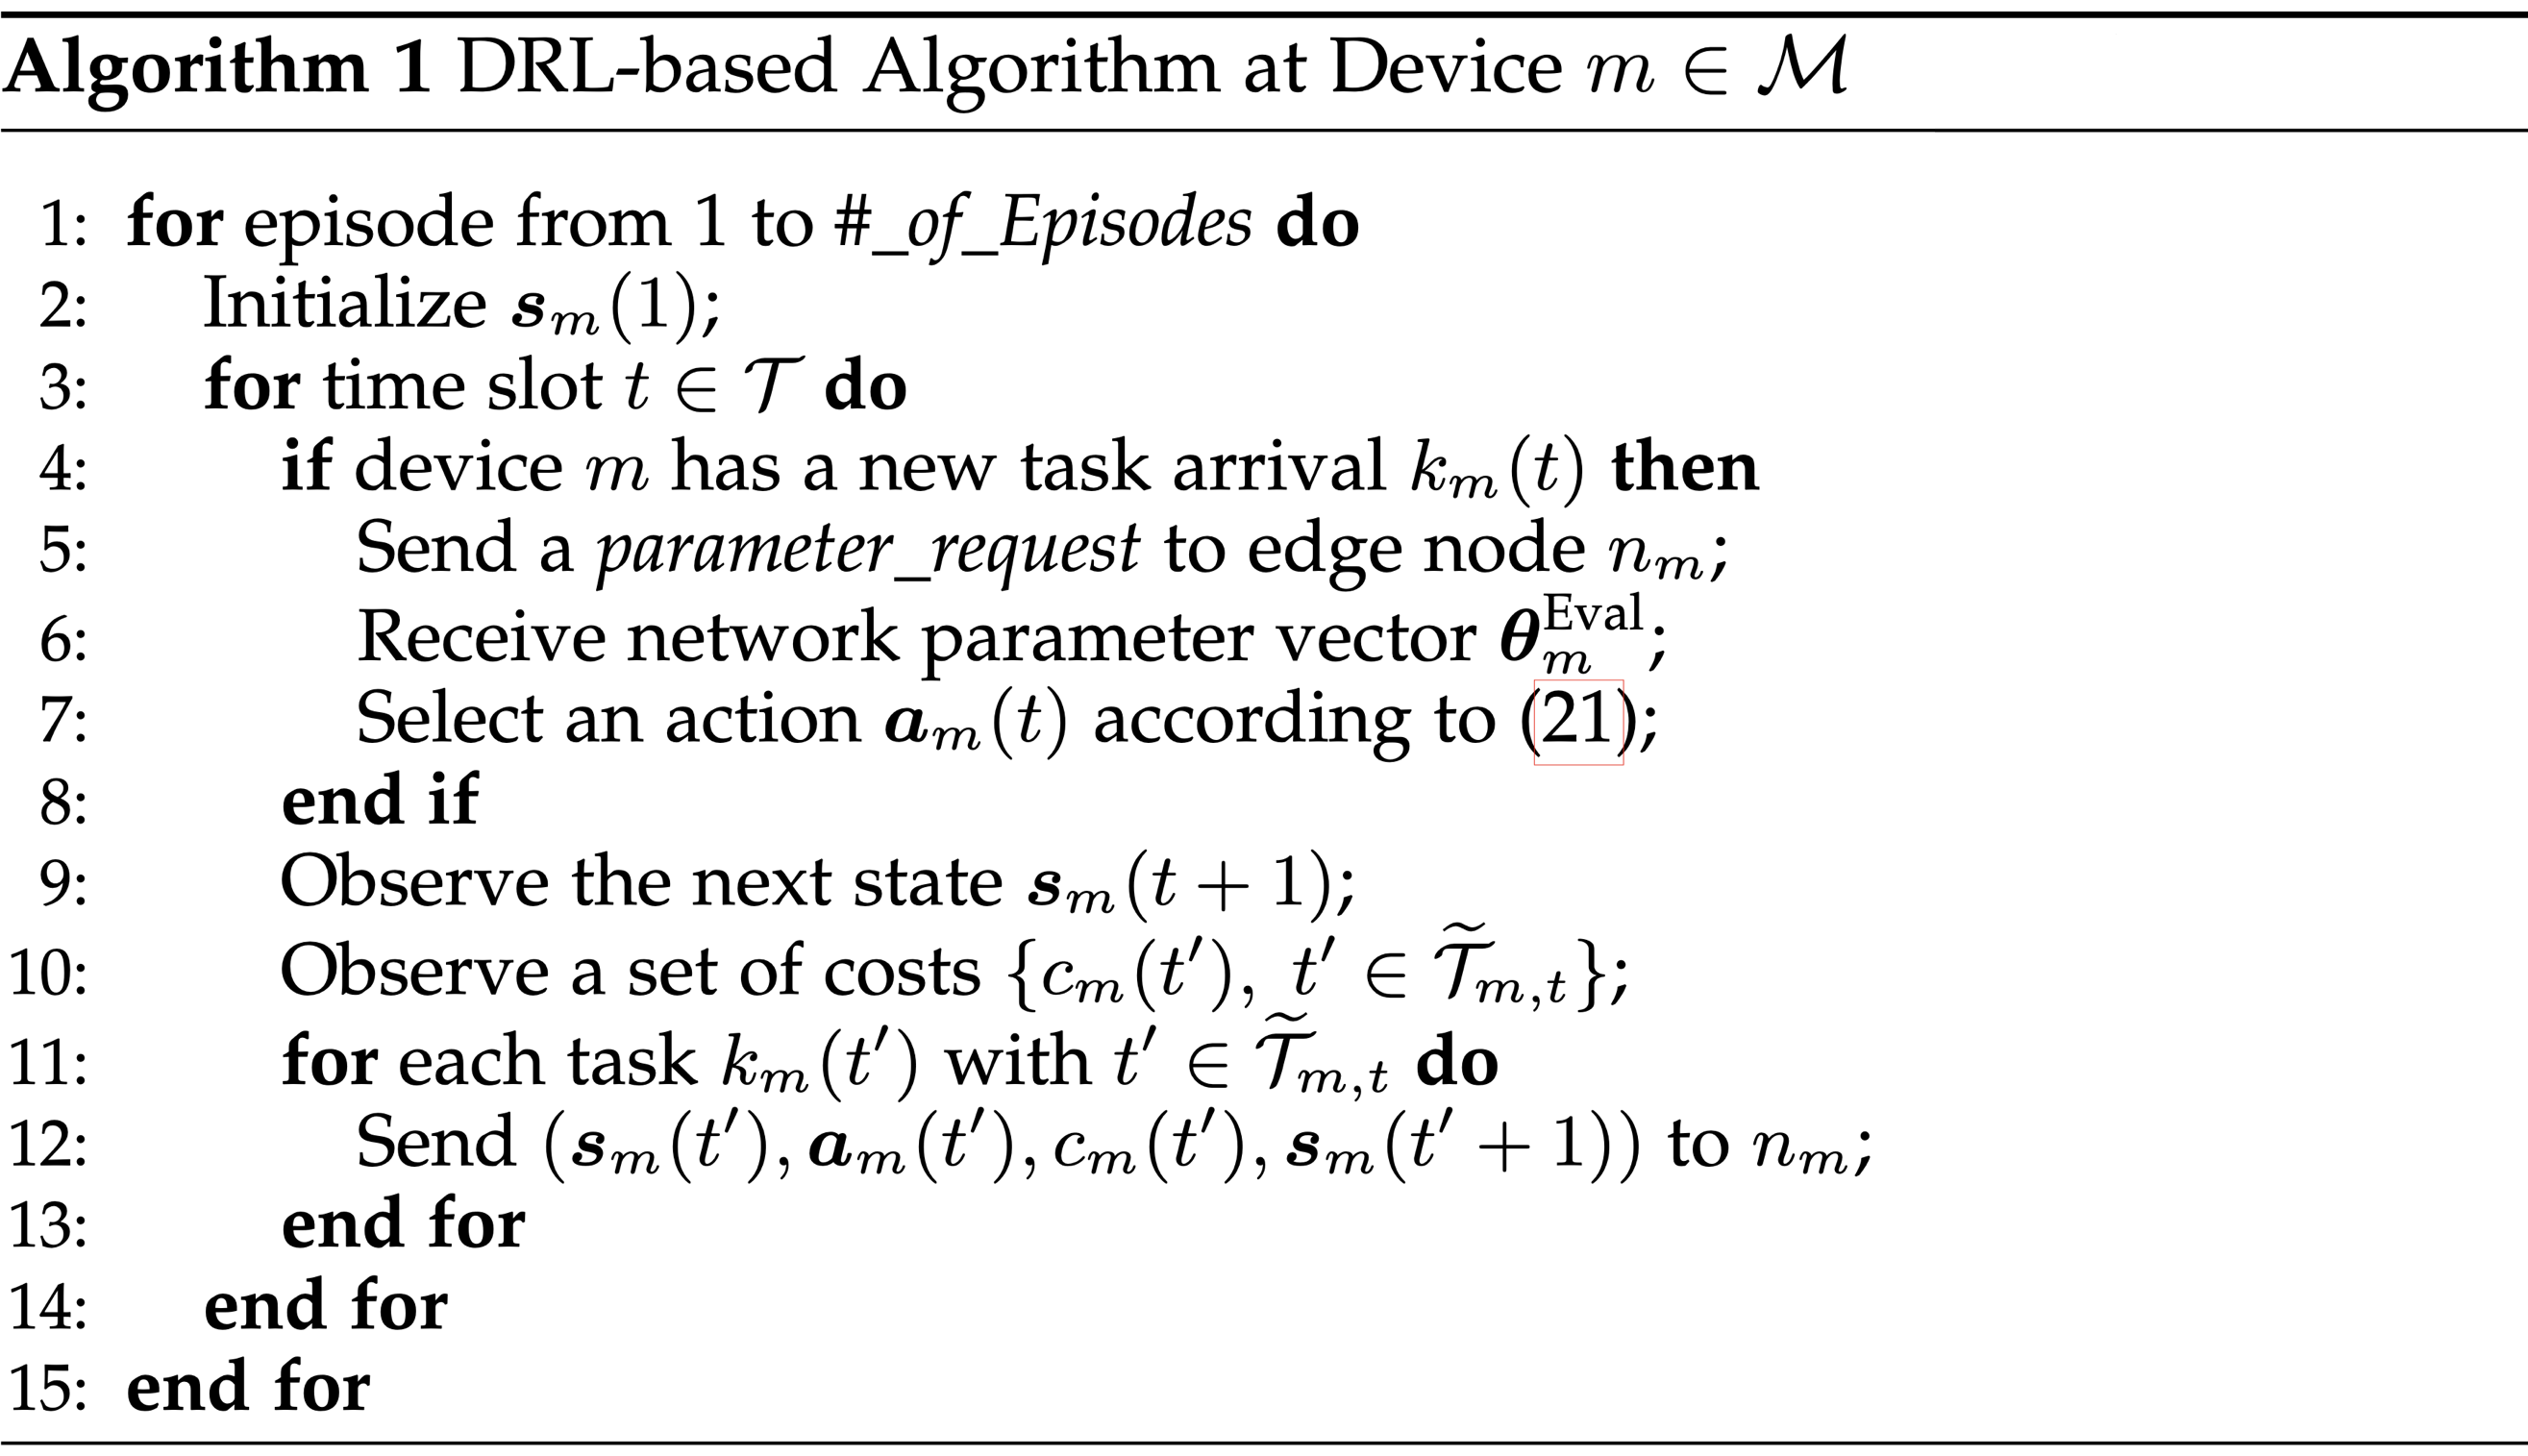
\includegraphics[width=]{all1.png}
%	\label{key}
%	\caption{text}
%\end{figure}
%



در هر دستگاه تلفن همراه $m \in \mathcal{M}$، متغیر $A_m(s_m(t), a;\theta_m)$ در جهت اشاره به ارزش مزیت‌عمل عمل $a$ در حالت  $s_m(t) \in \mathcal{S}$ همراه با بردار مقادیر $\theta_m$ شبکه، تعریف می‌کنیم. شبکه ارزش حاوی یک شبکه کاملا متصل با مجموعه‌ای از نورون‌ها است، که به عنوان مسئول یادگیری ارزش حالت عمل می‌کند. برای هر دستگاه تلفن همراه $m$، متغیر $V_m(s_m(t);\theta_m)$ به عنوان ارزش حالت در حالت $s_m(t)$ همراه با بردار وزنی شبکه $\theta_m$، تعریف می‌کنیم. مقادیر $V_m(s_m(t);\theta_m)$ و $A_m(s_m(t);\theta_m)$ توسط پارامترهای بردار وزنی $\theta_m$ و ساختار شبکه عصبی از لایه ورودی تا لایه ارزش‌مزیت، تعیین می‌شود، به شکلی که بردار $\theta_m$ قابل تنظیم است و در الگوریتم مبتنی بر یادگیری تقویتی عمیق آموزش داده می‌شود.

بر اساس ساختار لایه ارزش‌مزیت، برای دستگاه تلفن همراه $m \in \mathcal{M}$، مقدار $Q$ حاصل از عمل $a \in \mathcal{A}$ تحت حالت $s_m(t) \in \mathcal{S}$ در لایه خروجی به صورت زیر محاسبه می‌شود:
\begin{alignat}{2}
	Q_m(s_m(t),a;\theta_m) = V_m(s_m(t);\theta_m) + \Bigg( A_m(s_m(t),a;\theta_m) - {1 \over |\mathcal{A}|} \sum\limits_{a^{'} \in \mathcal{A}}(A_m(s_m(t),a^{'};\theta_m) \Bigg)
	\label{60}  
\end{alignat}

که مجموع مقادیر ارزش‌حالت، تحت حالت مربوطه و مزیت‌عمل، طبق عمل مربوطه است (یعنی تفاوت بین ارزش مزیت‌عمل مربوطه نسبت به میانگین همه اقدامات).

به طور خلاصه، از لایه ورودی تا لایه خروجی، شبکه عصبی دستگاه تلفن همراه $m \in \mathcal{M}$ با بردار پارامتر $\theta_m$ یک نگاشت از جفت عملکرد حالت و مقادیر $Q$ را تشکیل می‌دهد (یعنی تحت هر حالت مشاهده شده $s_m(t) \in \mathcal{S}$، یک مقدار $Q$ برای هر اقدام $a \in \mathcal{A}$ وجود دارد که با $Q_m(s_m(t),a;\theta_m)$ نشان داده می‌شود)، که مشخص‌کننده هزینه طولانی مدت مورد انتظار در حالت مشاهده‌شده و هر یک از اقدامات در فضای عمل است.





\قسمت{الگوریتم مبتنی بر یادگیری تقویتی عمیق}

در الگوریتم مبتنی بر یادگیری تقویتی عمیق پیشنهادی، ما از گره‌های لبه برای کمک به دستگاه‌های تلفن همراه استفاده می‌کنیم، تا در جهت کاهش بارهای محاسباتی در دستگاه‌های تلفن همراه،  شبکه عصبی را آموزش‌دهند. به طور خاص برای هر دستگاه تلفن همراه $m \in \mathcal{M}$، یک گره لبه $n_m \in \mathcal{M}$ وجود دارد که به دستگاه $m$ در آموزش شبکه کمک می‌کند. این گره لبه می‌تواند گره‌ با بیش‌ترین ظرفیت محاسباتی در نظر گرفته‌شود. برای راحتی در ارائه، متغیر  $\mathcal{M}_n \subset \mathcal{M}$ را در اشاره به مجموعه دستگاه‌های تلفن همراه که از گره لبه $n \in \mathcal{N}$ در نظر می‌گیریم، به شکلی که $\mathcal{M}_n = \set{m \in \mathcal{M}|n_m = n}$.

لازم به توجه است که منطقی است که از گره‌های لبه مستقیماً در جهت آموزش شبکه بهره‌گیریم، به این علت که تبادل اطلاعات درگیر در آموزش (شامل اطلاعات وضعیت و پارامترهای شبکه عصبی) محدود است و علاوه بر این، ظرفیت محاسباتی مورد نیاز آموزش در هر دوره زمانی بسیار کمتر از وظایف دستگاه‌های تلفن همراه می‌باشد.

الگوریتم مبتنی بر یادگیری تقویتی عمیق در دستگاه تلفن همراه $m \in \mathcal{M}$ و گره لبه $n \in \mathcal{N}$ بر طبق الگوریتم ۱ و ۲ اجرا می‌شود. ایده کلیدی این الگوریتم آموزش شبکه عصبی با استفاده از تجربه دستگاه تلفن همراه (به عنوان مثال، حالت، عمل، هزینه و حالت بعدی)، برای به‌دست ‌آوردن نگاشتی از جفت عمل‌حالت به مقادیر $Q$ است، که براساس آن دستگاه می‌تواند اقدامی را انتخاب کند که منجر به کمینه‌کردن مقدار $Q$ در حالت مشاهده‌شده شود، تا هزینه طولانی‌مدت مورد انتظار آن به حداقل برسد.


در الگوریتم مبتنی بر یادگیری تقویتی عمیق، در گره لبه $n \in \mathcal{N}$، یک حافظه پخش‌مجدد $D_m$ و دو شبکه عصبی برای دستگاه متصل $m \in \mathcal{M}_n$ نگه داشته می‌شود. حافظه بازپخش $D_m$ تجربه مشاهده شده $(s_m(t), a_m(t), c_m(t), s_m(t+1))$ دستگاه تلفن همراه $m$ را برای دوره زمانی $t \in \mathcal{T}$ ذخیره می‌کند، و این تجربه در حافظه بازپخش برای آموزش شبکه‌های عصبی استفاده می‌شود. همچنین دو شبکه عصبی شامل شبکه هدف ($Target\rule{0.25cm}{0.15mm}Net_m$) و شبکه ارزیابی ($Eval\rule{0.25cm}{0.15mm}Net_m$) است و مقادیر $Q$ توسط $Q_m^{Eval}(s_m(t), a; \theta_m^{Eval})$ و $Q_m^{Target}(s_m(t), a; \theta_m^{Target})$ تحت مشاهده حالت $s_m(t) \in \mathcal{S}$ و عمل $a \in \mathcal{A}$ بیان می‌شوند. توجه داشته باشید که $Eval\rule{0.25cm}{0.15mm}Net_m$ و $Target\rule{0.25cm}{0.15mm}Net_m$ ساختار شبکه عصبی مشابهی دارند، در حالی که آنها به ترتیب بردارهای پارامتر شبکه $\theta_m^{Eval}$ و $ \theta_m^{Target}$ را دارند. شبکه ارزیابی برای انتخاب عمل و شبکه هدف برای مشخص‌کردن یک مقدار هدف $Q$ استفاده می‌شود، که هزینه طولانی‌مدت مورد انتظار یک اقدام تحت وضعیت مشاهده‌شده را تقریب می‌زند. این مقدار هدف $Q$ برای به‌روز رسانی بردار پارامتر شبکه $\theta_m^{Eval}$ در  $Eval\rule{0.25cm}{0.15mm}Net_m$ با به حداقل رساندن اختلاف بین مقادیر $Q$ در $Eval\rule{0.25cm}{0.15mm}Net_m$ و مقادیر $Q$ هدف استفاده می‌شود. مقداردهی اولیه حافظه بازپخش $D_m$ و دو شبکه عصبی در مراحل $1$ تا $3$ در الگوریتم $2$ آورده شده‌است. در ادامه، الگوریتم مبتنی بر یادگیری تقویتی عمیق را به ترتیب در دستگاه تلفن همراه $m \in \mathcal{M}$ و گره لبه $n \in \mathcal{N}$ ارائه می‌کنیم.

\زیرقسمت{الگوریتم اجرایی در دستگاه تلفن همراه}

متغیر $Episodes$ را در اشاره به تعداد قسمت‌ها تعریف می‌کنیم. در ابتدای هر قسمت، دستگاه تلفن همراه $m \in \mathcal{M}$، وضعیت حالت را مطابق زیر مقداردهی اولیه می‌کند.
\begin{alignat}{2}
	\textbf{s}_m(1)=\Big(\lambda_m(1), \Delta(t)^{comp}(1), \Delta(t)^{tran}(1), \textbf{\textit{q}}_m^{edge}(0), \textbf{\textit{H}}(1) \Big)
	\label{61}  
\end{alignat} 



متغیر $\eta_{m,n}^{\text{E}}(0)$ را برای همه گره‌های لبه برابر با صفر قرار می‌دهیم و همچنین مقادیر ماتریس $\textbf{H}(1)$ را نیز در ابتدا برابر با صفر قرار می‌دهیم. هر قسمت شامل مجموعه‌ای از دوره‌های زمانی $\mathcal{T}$ است. 
در شروع دوره زمانی $t \in \mathcal{T}$، اگر دستگاه تلفن همراه $m$ یک وظیفه ورودی $k_m(t)$ داشته‌باشد، آنگاه درخواست پارامتر $(parameter \rule{0.25cm}{0.15mm} request)$ را به گره لبه $n_m$ ارسال می‌کند. پس از دریافت درخواست توسط گره لبه، بردار پارامتر $\theta_m^{Eval}$ شبکه $Eval\rule{0.25cm}{0.15mm}Net_m$ برای دستگاه ارسال می‌شود. سپس دستگاه $m$ برطبق رابطه زیر برای وظیفه $k_m(t)$، به انتخاب عمل می‌پردازد. 

\شروع{شکل}
\centerimg{all1}{15cm}
\پایان{شکل}



\شروع{شکل}[hb]
\centerimg{formol}{10cm}
\پایان{شکل}




در رابطه بالا، $\epsilon$ احتمال اکتشاف تصادفی را نشان می‌دهد. مقدار $Q_m^{Eval}(s_m(t), a; \theta_m^{Eval})$ برابر است با مقدار $Q$ تحت پارامترهای جاری $\theta_m^{Eval}$  از شبکه عصبی $Eval\rule{0.25cm}{0.15mm}Net_m$. به‌طور شهودی، با احتمال$1 - \epsilon$، دستگاه تلفن همراه عملی را انتخاب میکند که با حداقل مقدار $Q$ در حالت مشاهده‌شده $s_m(t)$، بر اساس $Eval\rule{0.25cm}{0.15mm}Net_m$ مطابقت دارد.

در ابتدای دوره زمانی بعدی (یعنی دوره زمانی $t+1$)، دستگاه تلفن همراه $m$ حالت بعدی $s_m(t+1)$ را مشاهده می‌کند. از سوی دیگر، از آنجایی که پردازش و انتقال یک وظیفه ممکن‌است برای چندین دوره زمانی ادامه‌یابد، هزینه $c_m(t)$ که به تأخیر وظیفه $K_m(t))$ بستگی دارد، ممکن‌است در ابتدای دوره زمانی جدید مشاهده نشود. 

همچنین دستگاه تلفن همراه $m$ ممکن‌است، مجموعه‌ای از هزینه‌های مربوط به برخی وظایف گذشته متعلق به وظیفه $k_m(t)$ را برای دوره زمانی $t \in \mathcal{T}$ مشاهده‌کند. در جهت رفع این مشکل، برای دستگاه $m$, $\Tilde{\mathcal{T}}_{m,t}} \subset \mathcal{T}$ را به عنوان مجموعه‌ای از دوره‌های زمانی تعریف می‌کنیم، به شکلی که هر وظیفه $K_m(t^{'})$ در دوره زمانی $t^{'}  \in \Tilde{\mathcal{T}}_{m,t}}$ پردازش‌شده یا در دوره زمانی $t$, منقضی شده‌است. مجموعه $\Tilde{\mathcal{T}}_{m,t}}$ در زیر تعریف شده‌است.

$\Tilde{\mathcal{T}}_{m,t}} = \Bigg\{ t^{'} \bigg| \ \ t^{'} = 1,2, \ldots, t, \  \  \lambda_m(t^{'})>0, x_m(t^{'})l_m^{\text{C}}(t^{'})   + \\ 1 - x_m(t^{'})) \sum\limits_{n \in \mathcal{N}} \sum\limits_{i = t^{'}}^{t}\mathds{1}(K_{m,n}^{edge}(i)=K_m(t^{'}))  l_{m,n}^{edge}(i) = t \Bigg\}$
\begin{alignat}{2}
	\text{ } \label{62}  
\end{alignat} 


در رابطه بالا، $\lambda_m(t^{'}) > 0$ به این معنی است که وظیفه ورودی جدید $K_m(t^{'})$ در دوره زمانی $t^{'}$ وجود دارد. به‌طورخاص مجموعه $\Tilde{\mathcal{T}}_{m,t}}$ شامل دوره‌های زمانی $t^{'} \in \set{1,2,\ldots,t}$ است. اگر وظیفه $K_m(t^{'})$ در دوره زمانی $t$ تکمیل‌شود، در ابتدای دوره زمانی $t+1$، دستگاه تلفن همراه $m$ مجموعه هزینه‌های $\set{c_m(t^{'}), t^{'} \in \Tilde{\mathcal{T}}_{m,t}}}$ را مشاهده می‌کند. سپس دستگاه $m$ برای هر وظیفه $K_m(t^{'})$ در دوره زمانی $t^{'} \in \Tilde{\mathcal{T}}_{m,t}}$، مشاهده خود را به گره لبه $n_m$ ارسال می‌کند. 







\زیرقسمت{الگوریتم اجرایی در گره لبه}


در ادامه پس‌از مقداردهی اولیه حافظه پخش‌مجدد $D_m$ و همچنین شبکه‌های عصبی $Eval\rule{0.25cm}{0.15mm}Net_m$ و $Target\rule{0.25cm}{0.15mm}Net_m$ برای دستگاه $m \in \mathcal{M}$، گره لبه $n \in \mathcal{N}$ منتظر پیام های درخواست از دستگاه های تلفن همراه در مجموعه Mn می شود.


اگر گره لبه $n \in \mathcal{N}$ درخواست پارامتر را از دستگاه تلفن همراه $m \in \mathcal{M}$ دریافت‌کند، آنگاه بردار پارامتر فعلی $Eval\rule{0.25cm}{0.15mm}Net_m$ را به دستگاه $m$ ارسال خواهدکرد. از سوی دیگر، اگر گره لبه $n$، تجربه $(s_m(t), a_m(t), c_m(t), s_m(t+1))$ را از دستگاه تلفن همراه $m \in \mathcal{M}_n$ دریافت‌کند، تجربه را در حافظه $D_m$ ذخیره می‌کند. حافظه به صورت اولین ورود، اولین خروج کار می‌کند. 


توجه داشته‌باشید که ما نیازی به همگام‌سازی بین دستگاه تلفن همراه $m$ و گره لبه مرتبط با آن $n_m$ نداریم. گره لبه شبکه عصبی را (در مراحل $10$ تا $20$‌ در الگوریتم $2$) آموزش می‌دهد تا بردار پارامتر $\theta_m^{Eval}$ از $Eval\rule{0.25cm}{0.15mm}Net_m$ را به‌صورت زیر به‌روزکند. 

\شروع{شکل}
\centerimg{all2}{15cm}
\پایان{شکل}

گره لبه به صورت تصادفی مجموعه‌ای از تجربیات را از حافظه نمونه‌برداری می‌کند (در مرحله $10$) که با $\mathcal{I}$ نشان داده شده‌است. بر اساس این نمونه‌های تجربه، ایده اصلی به‌روزرسانی $Eval\rule{0.25cm}{0.15mm}Net_m$، کمینه‌کردن تفاوت بین مقادیر $Q$ در $Eval\rule{0.25cm}{0.15mm}Net_m$ و مقادیر$Q$ هدف براساس نمونه‌های تجربه تحت شبکه هدف $Target\rule{0.25cm}{0.15mm}Net_m$ ‌است. 

به‌طور خاص برای یک تجربه نمونه در مجموعه $\mathcal{I}$، گره لبه $\hat{Q}_m^{Target} = (\hat{Q}_{m,i}^{Target} , i \in \mathcal{I})$ را محاسبه‌کرده و پارامتر $\theta_m^{Eval}$ در شبکه $Eval\rule{0.25cm}{0.15mm}Net_m$ برای کمینه‌کردن تابع زیان زیر به‌روزرسانی می‌کند.
\begin{alignat}{2}
	L(\theta_m^{Eval},\hat{Q}_m^{Target}) = {1 \over |\mathcal{I}| } \sum\limits_{i \in \mathcal{I}} \bigg(\hat{Q}_m^{Eval}(s_m(i) , a_m(i); \theta_m^{Eval} ) -   \hat{Q}_m^{Target}  \bigg)^2
	\label{63}  
\end{alignat}  





در رابطه بالا $|\mathcal{I}|$ کاردینالیتی مجموعه $\mathcal{I}$ است. تابع زیان، شکاف بین مقدار $Q$ با عمل $a_m(i)$ در حالت $s_m(i)$ تحت بردار شبکه $\hat{Q}_m^{Target}$ و مقدار $Q$ هدف $\hat{Q}_{m,i}^{Target}$ را برای هر تجربه در مجموعه $\mathcal{I}$ مشخص می‌کند. کمینه‌سازی تابع زیان با انجام یک مرحله گرادیان نزولی بر روی شبکه عصبی $Eval\rule{0.25cm}{0.15mm}Net_m$ با استفاده از انتشار پس‌انداز انجام می‌شود (به بخش 6 در~\cite{gers2000learning} مراجعه کنید).


مقدار $\hat{Q}_m^{Target}$ برای هر تجربه $i \in \mathcal{I}$، بر اساس تکنیک شبکه $Q$ عمیق دوگانه~\cite{wang2016dueling} تعیین می‌شود. تکنیک شبکه $Q$ عمیق دوگانه می‌تواند تخمین هزینه بلندمدت مورد انتظار را در مقایسه با روش‌های سنتی بهبود ببخشد. مقدار $\hat{Q}_m^{Target}$ برای تجربه $i$، مجموع هزینه متناظر در تجربه $i$ و مقدار $Q$ تنزیل‌شده عملی است که احتمالاً با توجه به وضعیت بعدی در تجربه $i$ تحت شبکه هدف $Target\rule{0.25cm}{0.15mm}Net_m$ ‌به شکل زیر انتخاب می‌شود.
\begin{alignat}{2}
	\hat{Q}_{m,i}^{Target} = c_m(i) + \gamma Q_m^{Target}(s_m(i+1)), a_i^{Next}; \theta_m^{Target})
	\label{64}  
\end{alignat}  

در رابطه بالا مقدار $a_i^{Next}$ نشان‌دهنده عملی است که کمترین مقدار $Q$ در حالت $s_m(i+1)$، تحت شبکه $Target\rule{0.25cm}{0.15mm}Net_m$ را به همراه خواهدداشت. 
\begin{alignat}{2}
	a_i^{Next} = arg \  \min\limits_{a \in \mathcal{A}} Q_m^{Eval}(s_m(i+1), a; \theta_m^{Eval})
	\label{65}  
\end{alignat}  





به طور شهودی، برای تجربه i، مقدار $Q$ هدف $\hat{Q}_{m,i}^{Target}$، هزینه طولانی مدت مورد انتظار عمل $a_m(i)$ در حالت $s_m(i)$‌ را نشان می‌دهد. این مقدار خلاصه‌ای از هزینه واقعی ثبت‌شده در تجربه $i$، یعنی $c_m(i)$ و همچنین هزینه تقریبی طولانی‌مدت مورد انتظار آینده بر اساس شبکه هدف $Target\rule{0.25cm}{0.15mm}Net_m$ یعنی $\gamma Q_m^{Target}(s_m(i+1)), a_i^{Next}; \theta_m^{Target})$ است. 


برای هر به‌روزرسانی $Replace\rule{0.25cm}{0.15mm}Threshold$، شبکه $Target\rule{0.25cm}{0.15mm}Net_m$ با کپی‌برداری از شبکه $Eval\rule{0.25cm}{0.15mm}Net_m$  توسط بردار پارامتر $\theta_m^{Eval}$ به‌روزرسانی می‌شود
 ($\theta_m^{Eval} = \theta_m^{Target}$).  


هدف از این مرحله، به‌روز نگه‌داشتن پارامتر شبکه $\theta_m^{Target}$ در $Target\rule{0.25cm}{0.15mm}Net_m$ است، به‌نحوی که بهتر می‌تواند هزینه طولانی‌مدت مورد انتظار را در محاسبه مقادیر هدف $Q$ تخمین‌بزند.







\فصل{نتایج}

در این فصل ابتدا جزییات سیستم شبیەسازی شده را شرح می‌دهیم و در ادامه به تحلیل نتایج به‌ دست‌‌آمده با توجه به معیارهای اصلی عملرد می‌پردازیم. 
\قسمت{شبیه‌سازی}

در این بخش نحوه پیاده‌سازی روش مبتنی بر یادگیری تقویتی عمیق پیشنهادی را شرح می‌دهیم. در جهت ارزیابی محیط مورد بررسی همانطور که در فصل $4$ اشاره‌شد، از شبیەسازی رخداد گسسته استفاده می‌کنیم.  در این شبیه‌سازی، نسبت وظایف منقضی‌شده به تعداد کل وظایف، میانگین تأخیر در وظایف تکمیل‌شده و انرژی مصرفی در کل سیستم را به عنوان سه معیار اصلی عملکرد در نظر می‌گیریم. و همچنین برای مقایسه عملکرد الگوریتم پیشنهادی، از سه روش معیار در سناریوهای چندگانه استفاده می‌کنیم. 



همانطور که در تنظیمات پارامترهای اصلی در جدول~\رجوع{جدول:تنظیمات پارامترها} آورده شده است، سناریویی را با 50 دستگاه تلفن همراه و ۵ گره لبه، شبیه‌سازی می‌کنیم. هر شکاف زمانی در شبیه‌سازی را برابر با $0.1$ ثانیه در نظر می‌گیریم و محیط را برای $‌100$ شکاف زمانی، معادل با $10$ ثانیه از زمان کار سیستم واقعی شبیه‌سازی می‌کنیم. در هر شکاف زمانی هر یک از دستگاه‌های تلفن همراه با احتمال $0.3$ وظیفه جدید ورودی دریافت می‌کنند، سپس باید تصمیم بگیرند که پردازش مربوط به وظیفه ورودی را خود بر عهده بگیرند و یا به گره لبه بارسپاری کنند. در حالتی که تصمیم بر بارسپاری باشد، دستگاه هوشمند می‌بایست گره لبه مناسب را با در نظر گرفتن پویایی سطح بار موجود انتخاب کرده و وظیفه ورودی را از طریق لینک ارتباطی موجود بارسپاری نماید.

\شروع{لوح}[t]
\تنظیم‌ازوسط

\شروع{جدول}{|c||c|}
\خط‌پر
\سیاه مقدار & \سیاه پارامتر \\ 
\خط‌پر \خط‌پر 
50 & $M$\\ 
\خط‌پر 
5 & $N$ \\ 
\خط‌پر 

$0.1$ ثانیه &  $\Delta(t)$ \\ 
\خط‌پر 
$2.5  \ GHz$ & $f_{m}^{device}, m \in \mathcal{M}$\\  \خط‌پر 
$41.8  \ GHz$ & $f_{‌n}^{edge}, n \in \mathcal{N}$\\  \خط‌پر 
$14  \ Mbps$ & $f_{m}^{tran}, m \in \mathcal{M}, n \in \mathcal{N}$\\  \خط‌پر 


$\set{2.0,2.1, \ldots, 5.0} \ Mbits$ & $\lambda_{m}(t), m \in \mathcal{M}, t \in \mathcal{T}$\\  \خط‌پر 
$0.297 \ gigacycles \ per \ Mbits$ & $\rho_m(t)(t)(t)(t)(t)(t)(t)(t)(t)(t)(t)(t)(t)(t)(t)(t)(t)(t)(t), m \in \mathcal{M}$\\  \خط‌پر 
$10$ واحد زمانی ($10 \times \Delta(t)$)  & $\tau_{m}, m \in \mathcal{M}$\\ \خط‌پر 
$0.2 W$ &  $\mathcal{P}^{\tetx{T}}$ \\  \خط‌پر 
$5 W$ &  $\mathcal{P}^{\text{E}}$ \\  \خط‌پر 
$1.5 W$ &  $\mathcal{P}^{\text{T}}(t)$ \\  \خط‌پر 
$0.03 W$ & $\mathcal{P}^{\text{I}}$  \\  \خط‌پر 

\پایان{جدول}

\شرح{تنظیمات پارامترهای اصلی}
\برچسب{جدول:تنظیمات پارامترها}
\پایان{لوح}


همچنین تنظیمات شبکه عصبی با اندازه دسته برابر با $16$ تنظیم شده‌است. نرخ یادگیری برابر با $0.001$ و ضریب تنزیل برابر با $0.9$ در نظر گرفته شده‌است و از طرفی احتمال کاوش تصادفی به تدریج از $1$ به $0$ کاهش می‌یابد. در این شبیه سازی‌ها ما بر روی یک سناریو با محیط ثابت تمرکز می کنیم، تابع انتقال (از حالت و عمل به حالت بعدی) و تابع هزینه (از حالت و عمل به هزینه) در طول زمان متغیر نیستند. در یک محیط غیر ثابت، اگر محیط تغییر کرده باشد، الگوریتم پیشنهادی می‌تواند با تنظیم مجدد احتمال اکتشاف تصادفی، به نحوی که اکتشاف تصادفی را دوباره فعال کند، با آن سازگار شود.







شبکه عصبی در الگوریتم پیشنهادی به صورت آنلاین آموزش داده می‌شود، به نحوی که تجربیات جمع‌آوری‌شده به صورت بی‌درنگ برای آموزش شبکه عصبی و به‌روزرسانی تصمیم‌گیری بارسپاری وظیفه استفاده می‌شود. این شبکه با بهره‌گیری از یادگیری ژرف و تقریب توابع می‌تواند مشکل رایج در این نوع از یادگیری یعنی نفرین ابعاد را مرتفع نماید. همچنین بهره‌گیری از تکنیک‌های شبکه یادگیری تقویتی $Q$ دوئل و دوگانه می‌تواند در یادگیری سیاست بهینه و سرعت همگرایی، بهبود قابل توجهی ایجاد کند. در راستای بررسی عملکرد الگوریتم پیشنهادی، همگرایی یادگیری را تحت فراپارامترهای مختلف شبکه عصبی و تنظیمات الگوریتم ارزیابی می‌کنیم. 






\قسمت{ارزیابی عملکرد}



در این بخش، به نحوه ارزیابی عملکرد روش ارايه‌شده پرداخته و در نهایت با تحلیل نتایج حاصل از شبیه‌سازی در شرایط متغیر به مقایسه عملکرد سیستم با سایر روش‌ها می‌پردازیم. 

در راستای بررسی عملکرد شبکه یادگیری تقویتی عمیق پیشنهادی، همگرایی یادگیری را تحت نرخ‌های یادگیری مختلف شبکه عصبی و تنظیمات تناوب به روز رسانی شبکه ارزیابی می‌کنیم. جهت ارزیابی عملکرد الگوریتم پیشنهادی با توجه به معیارهای اصلی عملکرد، نتایج حاصل از روش ارائه‌شده را در مقایسه با روش‌های معیار می‌سنجیم. همانطور که اشاره‌شد معیارهای عملکرد مورد توجه در این پژوهش شامل \textbf{نرخ وظایف منقضی‌شده}, \textbf{میانگین تأخیر در وظایف تکمیل‌شده} و \textbf{انرژی مصرفی در کل سیستم} می‌باشند، که در مقایسه الگوریتم پیشنهادی با روش‌های معیار استفاده می‌شوند. از این رو با توجه به محیط مورد بررسی و سناریوهای شبیه‌سازی شده، روش‌های مورد بررسی، به شکل زیر در نظر گرفته می‌شوند.
\شروع{فقرات}
\فقره $\textbf{روش محاسبات محلی:}$ این روش تنظیماتی از سیستم را نشان می‌دهد که در آن همه دستگاه‌های تلفن همراه موجود در سناریوی شبیه‌سازی شده، سعی می‌کنند تمامی وظایف خود را به صورت محلی و تحت حداکثر تأخیر قابل تحمل اجرا کنند. این روش در بخش مقایسه نتایج به اختصار به شکل (No-Offl) نشان داده شده‌است. 

\فقره $\textbf{روش بارسپاری تصادفی:}$ این روش تنظیماتی از سیستم را نشان می‌دهد که همه دستگاه‌های تلفن همراه متصل در شبیه‌سازی، وظایف خود را به صورت تصادفی در هر مرحله به یکی از گره‌های لبه در دسترس بارسپاری می‌کنند. در این حال کل منابع ارتباطی و محاسباتی گره لبه به طور مساوی به هر دستگاه‌های تلفن همراه اختصاص داده می‌شود. این روش در بخش مقایسه نتایج، به اختصار به شکل (Rand-Offl) نشان داده شده‌است. 

\فقره$\textbf{روش بارسپاری وظیفه برخط در سطح کاربر:}$
روش بارسپاری وظیفه ارایه‌شده در~\cite{neto2018uloof}, نسخه‌ای توسعه یافته جهت بارسپاری وظایف برخط در سطح کاربر است، به نحوی که می‌تواند سناریوهایی را با چند گره لبه، برای استقرار وظایف در نظر بگیرد. این روش بر اساس برآورد ظرفیت منابع با توجه به مشاهدات تاریخی طراحی شده است، که می‌تواند با بهینه‌سازی تصمیمات بارسپاری وظیفه به بهبود عملکرد سیستم دست‌یابد. این روش را جهت مقایسه نتایج حاصل از الگوریتم پیشنهادی انتخاب می‌کنیم، زیرا بسیار مشابه پژوهش ما بوده، و وظایف را به شکلی غیرقابل تقسیم و با مهلت زمانی در نظر می‌گیرد. همچنین بدون دخالت هیچ موجودیت متمرکزی سیستم را بررسی می‌نماید. این روش در بخش مقایسه  نتایج به اختصار به شکل (ULOOF) نشان داده شده‌است. 

%% در این حالت تصمیم‌گیری بارسپاری وظیفه با هدف به حداقل رساندن همزمان نرخ وظایف منقضی‌شده، میانگین تأخیر و مصرف انرژی در کل سیستم توسط شبکه یادگیری $Q$ پایه انجام می‌شود. ‌منابع سرور لبه به طور مساوی به هر دستگاه‌های تلفن همراه که بارسپاری وظیفه را انجام‌داده، تخصیص می‌یابد.

\فقره $\textbf{روش بارسپاری وظیفه مبتنی بر یادگیری $Q$ عمیق پیشنهادی:}$
روش پیشنهادی با بهره‌گیری از یادگیری تقویتی، به تعیین محل انجام محاسبات مربوط به هر وظیفه، در هر یک از دستگاه‌های هوشمند می‌پردازد. از این رو با هدف به حداقل رساندن معیارهای اصلی، می‌تواند با بهینه‌سازی هزینه سیستم به ایجاد تعادلی در برآورد نیازهای دستگاه‌های متصل دست‌یابد. در این روش الگوریتم پیشنهادی با استفاده از شبکه $Q$ عمیق دوئل، و تکنیک‌های شبکه $Q$ عمیق دوگانه می‌تواند از نفرین ابعاد حالات اجتناب‌کند و با بهبود هزینه‌های طولانی مدت و بهبود تصمیمات پیاپی، نیازهای وظایف ورودی را بر طرف نماید. روش پبشنهادی در بخش مقایسه نتایج به اختصار به شکل (P-DDQN) نشان داده شده است. 
\پایان{فقرات}

جهت آموزش شبکه یادگیری تقویتی عمیق، الگوریتم پیشنهادی را در $1000$ قسمت اجرا کرده و برای هر قسمت $100$ شکاف زمانی در نظر می‌گیریم، سپس در انتهای هر قسمت مقادیر هزینه و معیارهای اصلی عملکرد را ثبت نموده و در ادامه به تحلیل و مقایسه نتایج می‌پردازیم.


\قسمت{مقایسه نتایج}


در اولین مرحله از نتایج شبیه‌سازی به بررسی رفتار تابع هزینه سیستم مطابق (\ref{57}) در طی یادگیری در هر قسمت می‌پردازیم، هزینه سیستم برای هر یک از دستگاه‌های هوشمند برابر با قرینه قدرمطلق مجموع وزن‌داری از مقادیر عملکردهای اصلی تعریف می‌شود، که شامل نرخ وظایف منقضی‌شده، میانگین تأخیر وظایف تکمیل‌شده و انرژی مصرفی کل سیستم در شکاف‌های زمانی سیستم می‌باشد. از آنجا که انرژی مصرفی در تابع ‌هزینه هر دستگاه شامل انرژی کل سیستم از جمله انرژی انتقال وظایف، انرژی محاسبات در تجهیزات کاربر و محاسبات در گره‌های لبه می‌باشد، شایان ذکر است با توجه به اینکه دریافت مقادیر انرژی مصرفی محاسبه‌شده مربوط به محاسبات  وظایف هر دستگاه از گره‌های لبه بار زیادی به سیستم اعمال می‌کند، از این رو این انرژی مصرفی مطابق با (\ref{113}) در خود دستگاه‌ محاسبه می‌شود. 

نتایج حاصل از شبیه‌سازی، به صورت میانگین مقادیر هزینه همه‌ی دستگاه‌های هوشمند در طی یادگیری در شکل~\رجوع{شکل: متوسط هزینه} نشان‌ داده شده‌است. محور افقی نمودار، قسمت را نشان‌داده و محور عمودی میانگین هزینه دستگاه‌های تلفن همراه و کل شکاف‌های زمانی در هر قسمت را نشان می‌دهد. ما عملکرد الگوریتم پیشنهادی را تحت تنظیمات مختلف و خط مشی تصادفی (که با Rand مشخص می‌شود)، رسم می‌کنیم، که در آن اقدامات به شکل تصادفی انتخاب می‌شوند.

\شروع{شکل}
\centerimg{cost_main_4}{15cm}
\شرح{همگرایی الگوریتم پیشنهادی تحت تغییرات نرخ یادگیری.}
\برچسب{شکل: متوسط هزینه}
\پایان{شکل}


شکل~\رجوع{شکل: متوسط هزینه} همگرایی الگوریتم پیشنهادی را تحت مقادیر مختلف نرخ یادگیری نشان می‌دهد، که با (lr) مشخص می‌شود، و بیانگر اندازه گام در هر تکرار برای حرکت به سمت حداقل تابع ضرر است. در حالتی که نرخ یادگیری برابر با ($10^{-3}$) در نظر گرفته‌شود، همگرایی نسبتاً سریعی را شاهد هستیم. اما وقتی نرخ یادگیری کوچک‌تر (یعنی $10^{-4}$) باشد، همگرایی با کندی همراه خواهد بود. همچنین هنگامی که نرخ یادگیری بزرگ‌تر (یعنی $ 10^{-‌2}$ و $10^{-1}$) باشد، هزینه افزایش می‌یابد، که ممکن است حتی بیشتر از سیاست تصادفی باشد.
 



همانطور که در بخش‌های قبلی بیان‌شد، از آنجا که برای تسهیل در یادگیری، دستگاه‌های هوشمند شبکه‌های عصبی خود را در گره‌های لبه آموزش می‌دهند، برای به روز رسانی وزن‌های شبکه عصبی خود، درخواست بردار پارامتر خواهند داشت. این به روزرسانی می‌بایست در دوره‌های ثابت از شکاف‌های زمانی انجام‌شود. در شکل~\رجوع{شکل: متوسط هزینه2}، تنظیماتی را در نظر می‌گیریم که در آن یک دستگاه تلفن همراه درخواست پارامتر را برای به‌روز رسانی پارامتر شبکه خود در تعداد مشخصی از شکاف‌های زمانی ارسال می‌کند (به عنوان مثال به ازای هر شکاف زمانی که دستگاه تلفن همراه یک وظیفه دریافت می‌کند). همانطور که در نمودار نشان داده شده است، ارسال درخواست در هر 100 شکاف زمانی تاثیر زیادی بر عملکرد الگوریتم در مقایسه با ارسال در هر شکاف زمانی ندارد. 

\شروع{شکل}
\centerimg{cost_main_6}{15.5cm}
\شرح{همگرایی الگوریتم پیشنهادی تحت تغییرات تناوب درخواست پارامتر به روز رسانی.}
\برچسب{شکل: متوسط هزینه2}
\پایان{شکل}


این به این دلیل است که آموزش شبکه عصبی در الگوریتم پیشنهادی بر اساس نمونه‌برداری تصادفی تجربیات در صف بازپخش است و تجربیات تازه به‌دست‌آمده تاثیر زیادی ایجاد نخواهند کرد. از این رو، الگوریتم می‌تواند درجه معینی از تأخیر را از نظر به روز رسانی شبکه عصبی برای انتخاب عمل تحمل کند. در نتیجه، به منظور کاهش سربار ارتباط، می توانیم فرکانس ارسال درخواست پارامتر را بدون تأثیر قابل توجهی بر عملکرد الگوریتم کاهش دهیم.







%%شایان ذکر است که منابع مورد نیاز وظایف محاسباتی در هر شکاف زمانی متفاوت و پویا است، یک دستگاه هوشمند خاص ممکن است به دلیل منابع محاسباتی بیش از حد مورد نیاز تحت محدودیت حداکثر تأخیر مجاز، قادر به اجرای کار وارد شده به صورت محلی نباشد. بنابراین، تفاوت کلیدی بین روش‌ پیشنهادی و روش‌های پایه در این است که روش‌ پیشنهادی می‌تواند تصمیم‌گیری‌های بارسپاری را به صورت پویا انجام‌دهد.





همانطور که اشاره‌شد، جهت ارزیابی عملکرد روش مبتنی بر یادگیری تقویتی عمیق پیشنهادی ‌(‌که با P-DDQN مشخص می‌شود.)، با سه روش از جمله بدون بارسپاری (که با No-Offl مشخص می‌شود.)، بارسپاری تصادفی (که با Rand-Offl مشخص می‌شود.) و روش بارسپاری مبتنی بر چارچوب برخط سطح کاربر (که با ULOOF مشخص می‌شود.) مطابق با~\cite{tang2020deep}، در سه معیار اصلی عملکرد از جمله نرخ وظایف منقضی‌شده (یعنی نسبت تعداد وظایف منقضی‌شده به تعداد کل وظایف واردشده به سیستم)، میانگین تأخیر (یعنی متوسط ​​تأخیر وظایفی که پردازش شده‌اند) و میزان مصرف انرژی در کل سیستم مقایسه می‌کنیم.


\شروع{شکل}
\centerimg{drrop}{15.5cm}
\شرح{مقایسه عملکرد در نرخ وظایف منقضی‌شده تحت: (a) تغییرات تعداد دستگاه‌های متصل و (b) تغییرات مقدار احتمال ورود وظیفه در هر شکاف زمانی.}
\برچسب{شکل: دراپ}
\پایان{شکل}


با توجه به معیارهای اصلی مورد ارزیابی در سیستم، تنظیمات سیستم را تحت تغییرات در تعداد دستگاه‌های متصل و تغییرات در احتمال ورود وظیفه در هر شکاف زمانی به آزمایش می‌گذاریم. در شکل~\رجوع{شکل: دراپ}، نمودار (‌a) رفتار نرخ وظایف منقضی‌شده را در مقایسه با تعداد دستگاه‌های متصل نشان داده، و نمودار (b) رفتار نرخ وظایف منقضی‌شده در مقایسه با احتمال ورود وظیفه در هر شکاف زمانی را نمایش می‌دهد. 

در شکل~\رجوع{شکل: دراپ}، الگوریتم پیشنهادی به نرخ پایین‌تری در وظایف منقضی‌شده نسبت به روش‌های دیگر دست می‌یابد، به خصوص زمانی که تعداد دستگاه‌ها زیاد باشد. این به این دلیل است که الگوریتم پیشنهادی می‌تواند به طور موثر، بار ناشناخته را در گره‌های لبه بررسی‌کند. هنگامی که تعداد دستگاه‌های تلفن همراه به $80$ دستگاه افزایش می‌یابد، الگوریتم پیشنهادی نرخ وظایف منقضی‌شده را کمتر از $‌‌0.1$ حفظ می‌کند. در نمودار (a) با افزایش تعداد دستگاه‌های تلفن همراه، میانگین تأخیر هر روش (به جز بدون بارسپاری) به دلیل افزایش بالقوه بار در گره‌های لبه افزایش می‌یابند. 

همچنین در نمودار (b) با افزایش احتمال ورود وظیفه، الگوریتم مبتنی بر یادگیری تقویتی عمیق پیشنهادی در همه احتمالات ورودی می‌تواند نسبت کمتری از وظایف منقضی‌شده را در مقایسه با روش‌های معیار حفظ کند. هنگامی که احتمال ورود وظیفه کوچک است (به عنوان مثال $0.1$) اکثر روش‌ها می‌توانند نسبت وظایف حذف‌شده را در حدود صفر به دست آورند. با افزایش احتمال ورود وظیفه از $0.1$ به $0.5$، نسبت وظایف منقصی‌شده در الگوریتم پیشنهادی کمتر از $0.2$ باقی می‌ماند، در حالی که روش‌های معیار به بیش از $0.5$ افزایش می یابد. 

\شروع{شکل}
\centerimg{delay}{15.5cm}
\شرح{مقایسه عملکرد در میانگین تأخیر تحت: (a) تغییرات تعداد دستگاه‌های متصل و (b) تغییرات مقدار احتمال ورود وظیفه در هر شکاف زمانی.}
\برچسب{شکل: دیلی}
\پایان{شکل} 

در شکل~\رجوع{شکل: دیلی}, نمودار (‌a) رفتار میانگین تأخیر را در مقایسه با تعداد دستگاه‌های متصل و نمودار (b) رفتار میانگین تأخیر را در مقایسه با احتمال ورود وظیفه در هر شکاف زمانی، نمایش می‌دهد. در نمودار (a) با افزایش تعداد دستگاه های تلفن همراه، میانگین تأخیر هر روش (به جز بدون بارسپاری) به دلیل افزایش بالقوه بار در گره‌های لبه افزایش می‌یابد. از آنجایی که الگوریتم پیشنهادی می‌تواند به طور موثر با پویایی بار لبه ناشناخته مقابله کند، وقتی تعداد دستگاه‌های تلفن همراه به $130$ دستگاه افزایش می‌یابد، می‌تواند به میانگین تأخیر کمتری از روش‌های معیار دست‌یابد.


در نمودار (b) نیز با افزایش احتمال ورود وظیفه از $0.1$ به $0.5$، میانگین تأخیر الگوریتم مبتنی بر یادگیری تقویتی عمیق پیشنهادی حدود $20$ درصد افزایش می‌یابد، در حالی که روش‌های معیار حداقل $32$ درصد افزایش می‌یابند. این نشان می‌دهد در حالی که بار سیستم افزایش می‌یابد، میانگین تأخیر الگوریتم پیشنهادی به طور چشمگیری کمتر از روش‌های معیار افزایش می‌یابد. همانطور که احتمال رسیدن کار به $0.6$ افزایش می‌یابد، میانگین تأخیر برخی از روش‌ها کاهش می‌یابد، زیرا تعداد فزاینده‌ای از وظایف منقضی می‌شوند و بنابراین در تأخیر متوسط ​​محاسبه نمی‌شوند. به همین دلیل، زمانی که بار سیستم زیاد است، الگوریتم پیشنهادی ممکن است تأخیر متوسط ​​بیشتری نسبت به روش‌های دیگر داشته باشد، زیرا وظایف کمتری منقضی می‌شوند. 




در شکل~\رجوع{شکل: انرژی}، نمودار (‌a) میزان مصرف انرژی کلی سیستم را در مقایسه با تعداد دستگاه‌های متصل و نمودار (b) میزان مصرف انرژی کلی سیستم را در مقایسه با احتمال ورود وظیفه در هر شکاف زمانی، نمایش می‌دهد. 

\شروع{شکل}
\centerimg{energy}{15.5cm}
\شرح{مقایسه عملکرد در مقدار انرژی مصرفی سیستم تحت: (a) تغییرات تعداد دستگاه‌های متصل و (b) تغییرات مقدار احتمال ورود وظیفه در هر شکاف زمانی.}
\برچسب{شکل: انرژی}
\پایان{شکل}


در نمودار(a) با افزایش تعداد دستگاه‌های تلفن همراه و در پی آن افزایش وظایف در سیستم، میزان مصرف انرژی در هر روش افزایش می‌یابد. با گسترش تعداد دستگاه‌های متصل از $‌10$  به $130$، میزان مصرف انرژی در روش بدون بارسپاری حدود $80$ واحد و در روش بارسپاری تصادفی حدود $‌210$ واحد، افزایش می‌یابد. در ابتدا با وجود کمتر از $80$ دستگاه متصل، میزان مصرف انرژی سیستم در روش بدون بارسپاری، بیش‌تر از روش بارسپاری تصادفی می‌باشد، این در حالی است که با وجود تعداد بیشتری از دستگاه‌ها در سیستم، میزان مصرف انرژی در روش بدون بارسپاری کم‌تر از روش بارسپاری تصادفی می‌باشد، این به این خاطر است که افزایش بار در سیستم سبب افزایش زمان محاسبات در گره‌های لبه و در نتیجه زمان انتظاری بیشتر در رابط کاربری تجهیزات کاربر خواهد بود، که این افزایش زمان انتظار سبب افزایش میزان انرژی مصرفی در سیستم می‌شود. از این رو از آنجایی که الگوریتم پیشنهادی می‌تواند به طور موثر با پویایی بار در سیستم تطبیق یابد، می‌تواند در مواجه با افزایش تعداد دستگاه‌های تلفن همراه، مصرف انرژی کمتری را از روش‌های معیار کسب‌کند. 


همچنین در نمودار (b) با افزایش احتمال ورود وظایف، میزان مصرف انرژی در هر روش افزایش می‌یابد. با افزایش حتمال ورود وظیفه از $‌0.1$  به $0.9$، میزان مصرف انرژی در روش بدون بارسپاری حدود $125$ واحد و در روش بارسپاری تصادفی حدود $‌210$ واحد، افزایش می‌یابد. در احتمالات ورود کمتر از $0.7$، میزان مصرف انرژی سیستم در روش بدون بارسپاری، بیش‌تر از روش بارسپاری تصادفی می‌باشد، این در حالی است که با احتمال ورود بیشتر، میزان مصرف انرژی در روش بدون بارسپاری کم‌تر از روش بارسپاری تصادفی می‌باشد. 

از آنجایی که افزایش تعداد دستگاه‌های متصل و افزایش احتمال ورود وظیفه، هر دو با افزایش تعداد وظایف همراه هستند در نتیجه رفتار نمودار (b) در روش بارسپاری تصادفی مشابه رفتار آن در نمودار (a) خواهد بود، اما در روش بدون بارسپاری، نرخ رشد انرژی مصرفی با افزایش احتمالات ورود، روند کاهشی خواهد یافت. این به این جهت است که ظرفیت محاسباتی تجهیزات کاربر اشباع خواهد شد و تعداد ‌وظایف منقضی‌شده افزایش خواهدیافت. در اینجا نیز الگوریتم‌های مبتنی بر تصمیم‌گیری می‌توانند به طور موثر با پویایی بار در سیستم تطبیق یابند و در مواجه با افزایش احتمال ورود وظیفه در دستگاه‌های تلفن همراه مقابله نمایند. از این رو می‌توانند مصرف انرژی بهینه‌تری را از روش‌های معیار داشته‌باشند. از این رو الگوریتم یادگیری عمیق پیشنهادی توانسته‌است به کاهش مصرف انرژی در کل سیستم دست‌یابد. 



%%%
 
%%در شکل ()، با افزایش مهلت انجام وظیفه، میانگین تأخیر هر روش افزایش‌یافته و به تدریج همگرا می‌شود. این به این دلیل است که وقتی مهلت بزرگ‌تر باشد، وظایفی که به زمان پردازش (و انتقال) بیشتری نیاز دارند، می‌توانند پردازش شوند و در تأخیر متوسط ​​محاسبه شوند. وقتی مهلت به اندازه کافی بزرگ باشد، هیچ وظیفه‌ای حذف نمی‌شود، بنابراین افزایش بیشتر مهلت تفاوتی ندارد. همانطور که در شکل () نشان داده شده‌است، میانگین تأخیر الگوریتم پیشنهادی پس از افزایش مهلت به $1.4$ ثانیه و میانگین تأخیر همگرا در حدود 0 است (به عنوان مثال، به افزایش حاشیه ای کمتر از $0.05$ دست می یابد) $54$ ثانیه در مقایسه، میانگین تأخیر همگرای روش‌های دیگر بزرگ‌تر از $0.84$ ثانیه است. همانطور که در شکل 6 () نشان داده شده است، الگوریتم پیشنهادی همیشه به نسبت کارهای منقضی‌شده کمتری نسبت به روش‌های معیار دست می‌یابند، به خصوص زمانی که مهلت وظیفه کوچک است. زمانی که مهلت کار $‌0.6$ ثانیه باشد، الگوریتم پیشنهادی نسبت وظایف منقضی‌شده را در مقایسه با روش‌های معیار به میزان $65.8$ و $79.3$ کاهش می‌دهد. 

 
 %%%

\فصل{نتیجه‌گیری}


در این پژوهش به بررسی چالش بارسپاری وظایف در یک سیستم محاسباتی لبه پرداخته و با هدف به حداقل رساندن میانگین تأخیر و مصرف انرژی در طولانی‌مدت یک الگوریتم بارسپاری توزیع‌شده ارائه می‌دهیم، که دستگاه‌های تلفن همراه را قادر می‌سازد تا تصمیم‌گیری بارسپاری وظایف خود را به شیوه‌ای غیرمتمرکز انجام‌دهند، در حالی که می‌توانند پویایی سطح بار ناشناخته را در گره‌های لبه در نظر گرفته و به بهینه‌سازی کارایی سیستم در مواجهه با وظایف غیرقابل تقسیم و حساس به تأخیر بپردازد. و این در حالی است که محدودیت تأخیر و ظرفیت محدود منابع نیز در نظر گرفته شده است. 

نتایج شبیه سازی نشان می‌دهد که در مقایسه با چندین روش موجود، الگوریتم پیشنهادی ما می تواند نسبت کارهای منقضی شده، میانگین تاخیر و میزان مصرف انرژی را کاهش دهد. این مزیت به ویژه زمانی قابل توجه است که وظایف حساس به تاخیر باشند، یا سطوح بار در گره های لبه بالا باشد.

در جهت بهبود کارایی سیستم به گسترش یک مسئله بهینه‌سازی در قالب یک مشکل کمینه‌سازی تأخیر، مصرف انرژی و نرخ منقضی شدن وظایف، با وجود محدودیت تأخیر می‌پردازیم، از این رو با توسعه روش ارایه‌شده در پژوهش~\cite{tang2020deep} با استفاده از فرآیند تصمیم‌گیری مارکوف توصیف رابطه بین سیاست‌های بارسپاری در محیط سیستم را انجام می‌دهیم. سپس از یک روش مبتنی بر یادگیری تقویتی برای کشف استراتژی بهینه استفاده می‌کنیم. این رو با استفاده از مدل مصرف انرژی ارایه‌شده در پژوهش~\cite{zhou2021deep} به توسعه روشی ترکیبی و ایجاد تعادلی از معیارهای موجود در روش پیشنهادی می‌پردازیم. از این جهت برای جلوگیری از نفرین ابعاد ناشی از افزایش نمایی فضای حالت یک روش یادگیری $Q$ عمیق را به‌کار می‌گیریم، که می‌تواند نتایج عددی اثربخشی را در سناریوهای مختلف به دست آورد.  

نتایج شبیه‌سازی نشان داد که روش پیشنهادی در مقایسه با چندین روش معیار، از جمله روش چارچوب بارسپاری برخط مطابق با پژوهش~\cite{neto2018uloof}، توانسته نتایج بهتری را کسب نماید. روش پیشنهادی می‌تواند نرخ وظایف منقضی‌شده، میزان مصرف انرژی در کل سیستم و میانگین تأخیر را کاهش‌دهد. این مزیت به ویژه زمانی قابل توجه است که وظایف به تأخیر حساس باشند یا سطوح بار در گره‌های لبه بالا باشد. با این وجود، رویکرد پیشنهادی دارای محدودیت‌هایی است که می‌توانند مورد بررسی قرار گیرند، که به عنوان پژوهش‌های آینده به شرح زیر مطرح شوند.

\textbf{پژوهش‌های آینده:} 
از محدودیت‌های موجود در الگوریتم پیشنهادی می‌توان به پیچیدگی و سربار بالای سیستم در مقیاس‌های بزرگ اشاره کرد. از آنجایی که به گره‌های لبه اجازه می‌دهیم به دستگاه‌های متصل کمک کنند تا شبکه‌های عصبی را آموزش دهند، مشکل سربار ارتباط و مقیاس‌پذیری به دلیل انتقال پارامتر شبکه عصبی ممکن است زمانی که شبکه عصبی بزرگ است نگران‌کننده باشد. همچنین با وجود محوریت تاخیر و مصرف انرژی در سیستم می‌توان دریافت کاهش و بهینه‌سازی مصرف انرژی زمانی بسیار تاثیرگذار خواهد بود که با محدودیت انرژی در دستگاه‌ها و گره‌های لبه مواجه باشیم. از این رو می‌توان با شبیه‌سازی بلندمدت از سیستم و با در نظر گرفتن محدودیت انرژی در دستگاه‌های متصل به ارزیابی سیستم پرداخته‌شود.  


از جهتی می‌توان با توجه بیشتر به نیازهای هر کار به توسعه الگوریتم پیشنهادی در جهت بهبود کیفیت تجربه مشتری پرداخت. جالب است که با وجود نتایج بهبود یافته در الگوریتم پیشنهادی، می‌توان مشاهده نمود، که همواره بده‌بستانی در هزینه تحمیلی سیستم متشکل از سه معیار عملکرد برقرار خواهد بود، به نحوی که می‌توان با حذف هر کدام از آن‌ها، بهبودهای چشمگیری را در دو معیار دیگر مشاهده‌کرد، و از طرفی می‌توان دریافت که همه‌ی دستگاه‌های متصل در سیستم می‌توانند نیازهای متفاوتی در هر زمان داشته‌باشند. به عنوان مثال اگر تجهیزات کاربری در مواجهه با اتمام انرژی تجهیزات خود باشد، احتمالا می‌تواند متحمل اندکی تأخیر در مقابل انجام وظایف بیشتر باشد، اما در حالتی دیگر ممکن است حساسیت به تأخیر مهم بوده و بتوان از میزان مصرف انرژی صرفه نظر کرد. از این رو بسیار کارامد خواهد بود اگر بتوان معیارهای عملکرد را در برابر کاربران مختلف، شخصی‌سازی نمود. 

می‌توان با در نظر گرفتن ترکیبی وزن‌دار از معیارهای اصلی عملکرد، به نحوی انحصاری، به محاسبه کیفیت خدمات پرداخت. همچنین می‌توان با وجود تاریخچه‌ای از‌ هر کاربر و شرایط محیط در هر زمان پیش‌بینی‌ای از نیاز کاربر بدست‌آورد و با توجه به آن وزن‌ هریک از معیارهای عملکرد را تعیین‌ نمود. این امر می‌تواند با آموزش چند شبکه عصبی جداگانه برای هر معیار و بهره‌گیری از یک مکانیسم توجه\پاورقی{Attention Mechanism} پیاده‌شود. 


همچنین از جهتی دیگر، کارآمد خواهد بود اگر مدل شبکه بی‌سیم ساده‌شده را گسترش دهیم تا جزئیات بیشتری را در محیط شبیه‌سازی شده دربر گیرد، به عنوان نمونه می‌توان با در نظر گرفتن خطای انتقال و تداخل بین دستگاه‌های تلفن همراه در ارتباطات به دقت واقع‌بینانه‌تری از سیستم دست‌یافت. همچنین می‌توان عملکرد الگوریتم را در یک سیستم آزمایشی ارزیابی کرد، که تحت آن بسیاری از مسائل عملی (به عنوان مثال، وظایف محاسباتی واقعی) مورد بررسی قرار گیرند. پیاده‌سازی می‌تواند با استفاده از شبیه‌سازهای مناسب انجام شود و الگوریتم پیشنهادی مورد ازیابی قرار گیرد. 



 
 

 


 

  
  
  
  
  
 
 
 
 





